\documentclass[times,specification,annotation]{itmo-student-thesis}

\usepackage{icomma}

\usepackage{tabularx}

\usepackage{amsmath}
\usepackage{tikz}
\usepackage{svg}
\usepackage{pdfpages}
\usetikzlibrary{arrows}
\usepackage{filecontents}
\graphicspath{ {./png/} }
\begin{filecontents}{bachelor-thesis.bib}
@article{ indirect-ga-nsp,
    author      = {Aickelin, Uwe and Dowsland, Kathryn A.},
    title       = {An Indirect Genetic Algorithm for a Nurse Scheduling Problem},
    journal     = {Computers \& Operations Research},
    year        = {2004},
    pages       = {761–778}
}

@InProceedings{10.1007/3-540-61794-9_66,
author="Cooper, Tim B.
and Kingston, Jeffrey H.",
editor="Burke, Edmund
and Ross, Peter",
title="The complexity of timetable construction problems",
booktitle="Practice and Theory of Automated Timetabling",
year="1996",
publisher="Springer Berlin Heidelberg",
address="Berlin, Heidelberg",
pages="281--295",
isbn="978-3-540-70682-3"
}

@article{doi:10.1177/0954411919889560,
author = {Mahdi Hamid and Reza Tavakkoli-Moghaddam and Fereshte Golpaygani and Behdin Vahedi-Nouri},
title ={A multi-objective model for a nurse scheduling problem by emphasizing human factors},
journal = {Proceedings of the Institution of Mechanical Engineers, Part H: Journal of Engineering in Medicine},
volume = {234},
number = {2},
pages = {179-199},
year = {2020},
doi = {10.1177/0954411919889560},
}

@INPROCEEDINGS{934319,

  author={Burke, E.K. and De Causmaecker, P. and Petrovic, S. and Berghe, G.V.},
  booktitle={Proceedings of the 2001 Congress on Evolutionary Computation (IEEE Cat. No.01TH8546)}, 
  title={Fitness evaluation for nurse scheduling problems}, 
  year={2001},
  volume={2},
  number={},
  pages={1139-1146 vol. 2},
  doi={10.1109/CEC.2001.934319}
}
@ARTICLE{996017,

  author={Deb, K. and Pratap, A. and Agarwal, S. and Meyarivan, T.},

  journal={IEEE Transactions on Evolutionary Computation}, 

  title={A fast and elitist multiobjective genetic algorithm: NSGA-II}, 

  year={2002},

  volume={6},

  number={2},

  pages={182-197},

  doi={10.1109/4235.996017}}
@article{doi:10.1057/palgrave.jors.2600970,
author = {K A Dowsland and J M Thompson},
title = {Solving a nurse scheduling problem with knapsacks, networks and tabu search},
journal = {Journal of the Operational Research Society},
volume = {51},
number = {7},
pages = {825-833},
year  = {2000},
publisher = {Taylor & Francis},
doi = {10.1057/palgrave.jors.2600970}
}
@article{BELLANTI200428,
title = {A greedy-based neighborhood search approach to a nurse rostering problem},
journal = {European Journal of Operational Research},
volume = {153},
number = {1},
pages = {28-40},
year = {2004},
note = {Timetabling and Rostering},
issn = {0377-2217},
doi = {https://doi.org/10.1016/S0377-2217(03)00096-1},
author = {F. Bellanti and G. Carello and F. {Della Croce} and R. Tadei},
keywords = {Nurse rostering, Tabu search, Iterated local search},
abstract = {A practical nurse rostering problem, which arises at a ward of an Italian hospital, is considered. The nurse rostering problem is a typical employee timetabling problem, where each month it is required to generate the nursing staff shifts subject to various contractual and operational requirements. These requirements may be in conflict especially for those months in which manpower is reduced due to seasonal holidays. It is required to consider both holidays planning and parametric contractual constraints, but no cyclic schedules and corresponding weekly patterns. A local search approach is introduced which is based on a neighborhood operating on partial solutions completed by means of a greedy procedure so as to avoid the generation of infeasible solutions. Both a tabu search procedure and an iterated local search procedure are proposed. The solutions computed by the proposed procedures compare well with respect to a straightforward lower bound and strongly outperform those manually generated in the hospital ward. The proposed approach is now currently used on site.}
}
@article{nsp_ilp,
author = {Widyastiti, Maya and Aman, Amril and Bakhtiar, Toni},
year = {2016},
month = {09},
pages = {933-940},
title = {Nurses Scheduling by Considering the Qualification using Integer Linear Programming},
volume = {14},
journal = {TELKOMNIKA (Telecommunication Computing Electronics and Control)},
doi = {10.12928/TELKOMNIKA.v14i3.2913}
}
@article{boyd2007branch,
  title={Branch and bound methods},
  author={Boyd, Stephen and Mattingley, Jacob},
  journal={Notes for EE364b, Stanford University},
  volume={2006},
  pages={07},
  year={2007},
  publisher={Citeseer}
}
@InProceedings{10.1007/BFb0056845,
author="Droste, Stefan
and Jansen, Thomas
and Wegener, Ingo",
editor="Eiben, Agoston E.
and B{\"a}ck, Thomas
and Schoenauer, Marc
and Schwefel, Hans-Paul",
title="On the optimization of unimodal functions with the (1+1) evolutionary algorithm",
booktitle="Parallel Problem Solving from Nature --- PPSN V",
year="1998",
publisher="Springer Berlin Heidelberg",
address="Berlin, Heidelberg",
pages="13--22",
abstract="We investigate the expected running time of the (1+1) EA, a very simple Evolutionary Algorithm, on the class of unimodal fitness functions with Boolean inputs. We analyze the behavior on a generalized version of long paths [6, 10] and prove an exponential lower bound on the expected running time. Thereby we show that unimodal functions can be very difficult to be optimized for the (1+1) EA. Furthermore, we prove that a little modification in the selection method can lead to huge changes in the expected running time.",
isbn="978-3-540-49672-4"
}
@inproceedings{10.1145/2739480.2754674,
author = {Braun, Marlon Alexander and Shukla, Pradyumn Kumar and Schmeck, Hartmut},
title = {Obtaining Optimal Pareto Front Approximations Using Scalarized Preference Information},
year = {2015},
isbn = {9781450334723},
publisher = {Association for Computing Machinery},
address = {New York, NY, USA},
doi = {10.1145/2739480.2754674},
abstract = {Scalarization techniques are a popular method for articulating preferences in solving multi-objective optimization problems. These techniques, however, have so far proven to be ill-suited in finding a preference-driven approximation that still captures the Pareto front in its entirety. Therefore, we propose a new concept that defines an optimal distribution of points on the front given a specific scalarization function. It is proven that such an approximation exists for every real-valued problem irrespective of the shape of the corresponding front under some very mild conditions. We also show that our approach works well in obtaining an equidistant approximation of the Pareto front if no specific preference is articulated. Our analysis is complemented by the presentation of a new algorithm that implements the aforementioned concept. We provide in-depth simulation results to demonstrate the performance of our algorithm. The analysis also reveals that our algorithm is able to outperform current state-of-the-art algorithms on many popular benchmark problems.},
booktitle = {Proceedings of the 2015 Annual Conference on Genetic and Evolutionary Computation},
pages = {631–638},
numpages = {8},
keywords = {multi-objective optimization, scalarization method, electromagnetism-like mechanism, preference-based approximation},
location = {Madrid, Spain},
series = {GECCO '15}
}
@article{zitzler2001spea2,
  title={SPEA2: Improving the strength Pareto evolutionary algorithm},
  author={Zitzler, Eckart and Laumanns, Marco and Thiele, Lothar},
  journal={TIK-report},
  volume={103},
  year={2001},
  publisher={Eidgen{\"o}ssische Technische Hochschule Z{\"u}rich (ETH), Institut f{\"u}r Technische~…}
}
@article{kapelan2005multiobjective,
  title={Multiobjective design of water distribution systems under uncertainty},
  author={Kapelan, Zoran S and Savic, Dragan A and Walters, Godfrey A},
  journal={Water resources research},
  volume={41},
  number={11},
  year={2005},
  publisher={Wiley Online Library}
}
@inproceedings{10.5555/2955239.2955289,
author = {Corne, David W. and Jerram, Nick R. and Knowles, Joshua D. and Oates, Martin J.},
title = {PESA-II: Region-Based Selection in Evolutionary Multiobjective Optimization},
year = {2001},
isbn = {1558607749},
publisher = {Morgan Kaufmann Publishers Inc.},
address = {San Francisco, CA, USA},
abstract = {We describe a new selection technique for evolutionary multiobjective optimization algorithms in which the unit of selection is a hyperbox in objective space. In this technique, instead of assigning a selective fitness to an individual, selective fitness is assigned to the hyperboxes in objective space which are currently occupied by at least one individual in the current approximation to the Pareto frontier. A hyperbox is thereby selected, and the resulting selected individual is randomly chosen from this hyperbox. This method of selection is shown to be more sensitive to ensuring a good spread of development along the Pareto frontier than individual-based selection. The method is implemented in a modern multiobjective evolutionary algorithm, and performance is tested by using Deb's test suite of `T' functions with varying properties. The new selection technique is found to give significantly superior results to the other methods compared, namely PAES, PESA, and SPEA; each is a modern multi-objective optimization algorithm previously found to outperform earlier approaches on various problems.},
booktitle = {Proceedings of the 3rd Annual Conference on Genetic and Evolutionary Computation},
pages = {283–290},
numpages = {8},
location = {San Francisco, California},
series = {GECCO'01}
}
@ARTICLE{6600851,

  author={Deb, Kalyanmoy and Jain, Himanshu},

  journal={IEEE Transactions on Evolutionary Computation}, 

  title={An Evolutionary Many-Objective Optimization Algorithm Using Reference-Point-Based Nondominated Sorting Approach, Part I: Solving Problems With Box Constraints}, 

  year={2014},

  volume={18},

  number={4},

  pages={577-601},

  doi={10.1109/TEVC.2013.2281535}}
@article{durillo2006jmetal,
  title={jMetal: A java framework for developing multi-objective optimization metaheuristics},
  author={Durillo, Juan J and Nebro, Antonio J and Luna, Francisco and Dorronsoro, Bernab{\'e} and Alba, Enrique},
  journal={Departamento de Lenguajes y Ciencias de la Computaci{\'o}n, University of M{\'a}laga, ETSI Inform{\'a}tica, Campus de Teatinos, Tech. Rep. ITI-2006-10},
  year={2006}
}
@inproceedings{buzdalov2014provably,
  title={A provably asymptotically fast version of the generalized Jensen algorithm for non-dominated sorting},
  author={Buzdalov, Maxim and Shalyto, Anatoly},
  booktitle={Parallel Problem Solving from Nature--PPSN XIII: 13th International Conference, Ljubljana, Slovenia, September 13-17, 2014. Proceedings 13},
  pages={528--537},
  year={2014},
  organization={Springer}
}
\end{filecontents}

\addbibresource{bachelor-thesis.bib}

\begin{document}


\includepdf{pdf/title.pdf}

\includepdf[pages={1-2}]{pdf/assignment.pdf}

\includepdf[pages={1-2}]{pdf/annotation.pdf}
\newcommand{\TheOnlyTruePageStyle}{fancy}
\pagestyle{\TheOnlyTruePageStyle}
\renewcommand{\headrulewidth}{0pt}
\renewcommand{\footrulewidth}{0pt}
\lhead{}
\chead{\thepage}
\rhead{}
\lfoot{}
\cfoot{}
\rfoot{}
\addtolength{\voffset}{3mm}
\addtolength{\headsep}{-3mm}
\setcounter{page}{4}
\pretocmd{\tableofcontents}{\begingroup\banhyphens}{}{}
\apptocmd{\tableofcontents}{\endgroup}{}{}

\tableofcontents

\startprefacepage

Из года в год требования к сервисам растут.
Уже сегодня от многих сервисов ожидается круглосуточная бесперебойная работа.
Такие же требования предъявляются в том числе и к службам поддержки.
В таких сервисах довольно важно распределить ресурсы операторов.
Например, в час пик на смену необходимо выйти большему числу исполнителей, чем ночью.

Поэтому на любом таком предприятии рано или поздно появляются как задача планирования, так и задача прогнозирования нагрузки.
Эти задачи может решать вручную руководитель команды операторов, но таким способом планирование может затянуться на несколько часов, а то и дней.
Автоматизация процесса планирования оптимизирует время руководителей, а также улучшит качество покрытия прогноза, поэтому задача актуальна и имеет практическое значение.
Целью данной работы будем считать оптимизацию управления ресурсами служб поддержки.

Задачи автоматизации решаются разработкой программного обеспечения.
Одной из задач данной работы является разработка алгоритма, автоматизирующего процесс планирования смен.
Важно, что алгоритм может контролировать начало смены сотрудника и ее длину, поэтому команды со свободным графиком не рассматриваются.
Также важно, что для поступающей нагрузки установлен некий максимальный уровень отклика, то есть работа не может быть отложена.

Под аналогичные требования к алгоритму попадает также и работа больниц.
Больные не могут ждать часами, пока к ним придет медсестра.
Также в каждый момент времени в больнице должна находиться хотя бы одна медсестра, на случай форс-мажора.
Поэтому разработанный алгоритм должен быть сравнен с решениями задачи планирования работы больниц.

Для расписаний больниц уже сформулирована модель (en. NSP, nurse scheduling problem или nurse rostering problem, задача планирования дежурств медсестер), которая уже довольно долго изучается (более 50 лет~\cite{indirect-ga-nsp}).
Под разные ограничения человечество придумало множество решений: некоторые находят глобальный оптимум, некоторые локальный.
Тем не менее было доказано, что планирование смен медсестер в больнице~--- NP-трудная задача~\cite{10.1007/3-540-61794-9_66}.
То есть поиск глобального оптимума займет неприемлемо много времени и необходимо оптимизировать алгоритм для поиска локального оптимума.

Тем не менее, решаемая в данной работе задача отличается от задачи планирования дежурств медсестер.
В задаче планирования дежурств медсестер обычно рассматривают только три шаблона смены~--- ночь, утро или вечер.
В то время как в данной работе рассматриваются такие расписания, в которых число шаблонов смен достигает сотен, причем для разных операторов эти шаблоны разные.
Более того, в данной работе требуется спланировать перерывы операторов, что не входит в условия задачи планирования дежурств медсестер.

В первой главе дадим определение задаче планирования дежурств медсестер, а также определим решаемую в данной работе задачу.
Также в первой главе существующие решения как для больниц, так и для служб поддержки.
Далее, во второй главе, рассмотрим реализованный алгоритм, обсудим его плюсы и минусы.
Рассмотрим возможные подходы к реализации алгоритма и выберем лучший.
В завершение, в третьей главе обсудим, как реализовать алгоритм на практике, а также сравним полученный алгоритм с другими решениями.

\chapter{Задача планирования дежурств}

\startrelatedwork
\section{Планирование дежурств медсестер}

Человечество не первый раз решает задачи планирования смен для работников.
Самая похожая задача на рассматриваемую в данной работе~--- это nurse scheduling problem (NSP).
У этой задачи много различных постановок, тем не менее они обычно не сильно отличаются.
Рассмотрим постановку NSP:

\begin{enumerate}
    \item день состоит из трех, возможно пересекающихся, временных отрезка (обычно, утро, вечер и ночь), которые далее будем называть шаблонами смен;
    \item дана команда медсестер, каждая из медсестер может иметь какие-то навыки, предпочтения, должность;
    \item дан горизонт планирования, на который нужно спланировать смены медсестер;
    \item необходимо для каждой медсестры спланировать расписание смен (начало и длительность каждой смены определяется шаблоном).
\end{enumerate}

Причем на полученное расписание накладываются некоторые ограничения.
В разных работах~\cite{doi:10.1057/palgrave.jors.2600970, BELLANTI200428, indirect-ga-nsp, doi:10.1177/0954411919889560, 934319} ограничения предлагаются разные, рассмотрим некоторые примеры:

\begin{enumerate}
    \item в день медсестра работает не более одной смены;
    \item максимальное число смен в неделю для каждой медсестры;
    \item для каждого шаблона смены задано минимальное число медсестер определенной должности;
    \item для каждой должности задана производительность в условных единицах, и для каждого шаблона смены задан прогноз работы в тех же условных единицах;
    \item минимальное и/или максимальное число последовательных рабочих/выходных дней;
    \item различия в ночных и дневных шаблонах смен: например, более строгое ограничение на число смен в неделю, если хотя бы одна из них ночная;
    \item для каждого шаблона смены задан набор навыков, которые имеют только определенные медсестры~--- для каждого навыка в шаблоне смены должно быть ненулевое число смен медсестер с этим навыком;
    \item для каждой пары медсестер задана совместимость~--- некоторые пары в совокупности работают лучше, некоторые хуже.
\end{enumerate}

Для решения такой проблемы существует множество решений: некоторые находят глобальный оптимум, некоторые~--- локальный (если в постановке задачи заданы мягкие ограничения~--- функции, которые нужно минимизировать или максимизировать).
Рассмотрим некоторые решения, а также их плюсы и минусы.

\subsection{Использование задачи о рюкзаке}

Рассмотрим один из способов разделить большую задачу на две задачи поменьше~\cite{doi:10.1057/palgrave.jors.2600970}.
Перед тем как описать способ, уточним постановку задачи планирования дежурств медсестер:

\begin{enumerate}
    \item для каждого шаблона смены известен один из типов~--- ночной шаблон или дневной шаблон смены;
    \item для каждой медсестры задан тип договора $t$;
    \item для каждого типа договора задано $d_t$ и $e_t$~--- сколько дневных и ночных смен в неделю может быть назначено на медсестру по договору $t$ соответственно;
    \item за неделю медсестра может работать либо только в ночные смены, либо только в дневные;
    \item в команде есть запасные медсестры, на которых можно назначать смены, если основной команды не хватает;
    \item для каждого шаблона смены задано минимальное число назначенных медсестер;
    \item число использованных запасных медсестер необходимо минимизировать.
\end{enumerate}

Просуммируем по всем дневным и ночным шаблонам смены минимальное число назначенных медсестер.
Пусть $D$, $E$~--- суммарное число необходимых медсестер для дневных и ночных шаблонов смен соответственно.
Также пусть $y_t$, $N_t$, $T$~--- число медсестер с договором типа $t$, назначенных на ночную смену, число медсестер с договором типа типа $t$ и число типов договоров соответственно.
Тогда запишем ограничения следующим образом:

\begin{equation} \sum\limits^T_{t=1}{e_t y_t} \ge E \label{knapsack_night_shifts_constraint}\end{equation}

\begin{equation} \sum\limits^T_{t=1}{d_t \left( N_t - y_t \right)} \ge D \label{knapsack_day_shifts_constraint} \end{equation}

\begin{equation} \forall t : y_t \le N_t \end{equation}

\begin{equation} \forall t : y_t \in \mathbb{Z}_+ \end{equation}

Применив преобразования к неравенству~\eqref{knapsack_day_shifts_constraint}, получим следующее

\begin{equation} \sum\limits^T_{t=1}{d_t y_t} \le \sum\limits^T_{t=1}{N_t d_t} - D \label{knapsack_day_shifts_constraint_improved}\end{equation}

Заметим, что в неравенствах~\eqref{knapsack_night_shifts_constraint} и~\eqref{knapsack_day_shifts_constraint_improved} правая часть постоянна, так как изменяется и оптимизируется лишь параметр $y_t$.
Иными словами, из правых частей выражения неравенств~\eqref{knapsack_night_shifts_constraint} и~\eqref{knapsack_day_shifts_constraint_improved} можно тривиально посчитать, имея входные данные.

Далее заметим, что $d_t$ можно считать весом предмета типа $t$ в контексте задачи о рюкзаке, $e_t$~--- стоимостью, а $y_t$~--- числом предметов типа $t$ в рюкзаке.
Таким образом, получим задачу об ограниченном рюкзаке, решение которой будет максимизировать левую часть~\eqref{knapsack_night_shifts_constraint}.
Если решение подберет недостаточно медсестер, добавим в команду несколько запасных медсестер и перезапустим алгоритм.
Пусть $C_i$~--- команда на $i$-й итерации, тогда получим следующее решение задачи:

\begin{enumerate}
    \item\label{enumerate:knapsack_algorithm_init_step} решить задачу о рюкзаке для команды $C_i$, получив $M_i = \max\limits_{y_{i, t}}{\sum\limits^T_{t=1}{e_{i, t} y_{i, t}}}$;
    \item если $M_i \ge E$, вернуть $y_{i, t}$;
    \item иначе добавить в команду $E - M_i$ запасных медсестер и перейти к шагу~(\ref{enumerate:knapsack_algorithm_init_step}).
\end{enumerate}

Таким образом, получим $y_t$, с помощью чего для каждой медсестры можно определить тип смен, в которые она будет работать.
Например, это можно делать жадным алгоритмом.
Далее можно решать задачу независимо для дневных и ночных смен, если это позволяют ограничения.

\subsection{Целочисленное линейное и квадратичное программирование} \label{milp_and_miqp_subsection}

Рассмотрим одно из решений задачи планирования дежурств медсестер~\cite{nsp_ilp}.
Заметим, что назначение на шаблон смены можно представить в виде логической переменной.
Пусть $a_{i, j} = 1$, если $i$-я медсестра назначена на $j$-й шаблон смены, иначе $a_{i, j} = 0$.
Тогда большинство ограничений задачи можно представить с помощью линейной комбинации.
Например, с помощью следующего равенства можно задать ограничение на ровно одну смену в первый день планируемого периода:

\begin{equation} a_{i, 1} + a_{i, 2} + a_{i, 3} = 1. \end{equation}

Аналогично, зададим ограничение на минимальное число медсестер, имеющих навык $g$.
Для простоты положим, что в первый шаблон смены должна быть хотя бы одна медсестра с навыком $g$.
Пусть $G = \{i \mid \text{медсестра}\; i\; \text{имеет навык}\; g \}$, тогда зададим ограничение для первого шаблона смены следующим образом

\begin{equation} \sum\limits_{i \in G} a_{i, 1} \ge 1. \end{equation}

В разных постановках задачи к расписанию предъявляются разные требования.
Иногда достаточно найти какое-то допустимое расписание, но часто при этом необходимо найти <<хорошее>> решение.
Формально, необходимо оптимизировать некоторую метрику в пространстве допустимых решений.
Например, в задаче часто заданы мягкие ограничения~--- функции, которые необходимо минимизировать для решения.
Если таких ограничений несколько, то необходимо их как-то агрегировать, например просуммировать.

Например, для каждого шаблона смены и медсестры может быть известен штраф, если у организации есть какие-то сведения о продуктивности медсестры по каждому периоду.
Аналогичное ограничение может быть задано при учете предпочтений медсестер.
Пусть $c_{i, j}$~--- штраф за назначение $i$-й медсестры на $j$-й шаблон смены (штраф может быть отрицательным).
Также пусть $S^T$ и $K$~--- число шаблонов смен и число медсестер соответственно, тогда зададим ограничение следующим образом

\begin{equation} \sum\limits_{i = 1}^{K}\sum\limits_{j = 1}^{S^T}{c_{i, j} a_{i, j}} \rightarrow \min \end{equation}

Рассмотренные выше ограничения описывают задачу целочисленного линейного программирования.
Такую задачу часто решают с помощью обычной задачи линейного программирования.
Для поиска целочисленного решения часто используют метод ветвей и границ~\cite{boyd2007branch}.

Рассмотрим метод ветвей и границ на примере поиска минимума функции.
Введем понятие релаксированной задачи линейного программирования.
В изначальной задаче $a_{i, j} \in \{0, 1\}$, в релаксированной же $a_{i, j} \in [0, 1]$.
Тогда релаксированную задачу можно решать методами обычного линейного программирования.

Рассмотрим как с помощью релаксированной задачи решить задачу целочисленного линейного программирования.
Для пространства $\mathcal{Q}$ и оптимизируемой функции $f$ поиска задается функция $\Phi(\mathcal{Q})$~--- минимум множества $f(\mathcal{Q})$ для релаксированной задачи.
Алгоритм инициализируется стартовым пространством поиска $\mathcal{Q}_0$ и каждую итерацию поддерживает семейство рассматриваемых множеств $\hat{\mathcal{Q}}$.
Также алгоритм поддерживает лучшее решение $a^b$, итеративно улучшая решение.
Будем считать, что все рассматриваемые множества являются гиперпрямоугольниками.
На каждой итерации необходимо выполнить следующие шаги:

\begin{enumerate}
    \item \label{enumerate:branch_and_bound_selection_step} выбрать множество $\mathcal{Q}_i$ из $\hat{\mathcal{Q}}$ и удалить его из семейства;
    \item если $\Phi(\mathcal{Q}_i)$ хуже, чем $a^b$, то вернуться к шагу~(\ref{enumerate:branch_and_bound_selection_step});
    \item \label{enumerate:branch_and_bound_division_step} разделить множество $\mathcal{Q}_i$ на $\mathcal{Q}_i^1$ и $\mathcal{Q}_i^2$;
    \item если $\Phi(\mathcal{Q}_i^k)$~--- целочисленное решение оптимальнее $a^b$, то обновить $a^b$ для $k \in \{1, 2\}$;
    \item добавить $\mathcal{Q}_i^1$ и $\mathcal{Q}_i^2$ в $\hat{\mathcal{Q}}$.
\end{enumerate}

Для реализации шага~(\ref{enumerate:branch_and_bound_selection_step}) можно псевдослучайно выбирать множество из семейства.
Также можно вычислять оценки на целочисленный минимум и выбирать множество с самой точной оценкой.
Для реализации шага~(\ref{enumerate:branch_and_bound_division_step}) можно фиксировать значение $a_{i, j}$ для каких-то $i$ и $j$, которые еще не были зафиксированы.
Например, для $\mathcal{Q}_i^1$ добавить ограничение $a_{i, j} = 0$, а для $\mathcal{Q}_i^2$~--- ограничение $a_{i, j} = 1$.

Иногда оптимизируемая функция нелинейна и линейное программирование не применимо.
Тем не менее, такую функцию иногда можно выразить квадратичной функцией~--- такую функцию можно оптимизировать методами целочисленного квадратичного программирования.

Рассмотрим плюсы данного подхода:

\begin{enumerate}
    \item алгоритм можно параллелизовать и даже реализовать для исполнения в распределенной системе, например, разделяя $\mathcal{Q}$ для каждого потока;
    \item алгоритм можно преждевременно остановить, если полученное решение устраивает пользователя.
\end{enumerate}

А также перечислим его минусы:

\begin{enumerate}
    \item задача экспоненциально растет от числа переменных, а их часто очень много;
    \item алгоритм может работать дольше обычного перебора, если решение существует только в релаксированной задаче.
\end{enumerate}

\subsection{Жадный алгоритм}

Рассмотрим жадный алгоритм~\cite{BELLANTI200428}, который делает очень мало предположений о структуре задачи.
Единственное предположение, которое алгоритм делает~--- решение можно численно оценить.
Основная идея алгоритма~--- итеративно добавлять самую лучшую по какому-то критерию смену так, что полученное расписание удовлетворяет ограничениям.
Сам критерий зависит от точной постановки задачи, но его можно считать независимо от жадного алгоритма.
Поэтому данный алгоритм подходит для любой постановки задачи планирования, если расписание можно численно оценить.

Рассмотрим один из примеров использования данного алгоритма~\cite{BELLANTI200428}.
Будем постепенно добавлять смену на каждый шаблон смены, начиная с первого шаблона в планируемом периоде.
Добавлять смену к шаблону будем пока полностью не покроем ограничения по медсестрам, либо пока не просмотрим всех доступных медсестер.
Для итеративного выбора лучшей медсестры на каждую смену будем использовать критерий честности $k_i$ по отношению к медсестрам.
Зададим критерий $k_i$ для медсестры $i$ следующим образом: пусть $t$, $S^c_{t, i}$~--- тип смены (утренняя, вечерняя или ночная) и число смен типа $t$ у медсестры $i$ за последние два месяца, тогда

\begin{equation} k_i = S^c_{t, i} \end{equation}

Тогда алгоритм назначит смену на ту медсестру, которая меньше всего работала в такой тип смены за последние два месяца.
Рассмотрим плюсы данного подхода:

\begin{enumerate}
    \item алгоритм можно реализовать для любой задачи, в которой решение можно численно оценить.
\end{enumerate}

А также перечислим его минусы:

\begin{enumerate}
    \item алгоритм работает довольно долго, так как на каждой итерации пересчитывает значение штрафа для каждой допустимой смены, алгоритм нельзя остановить в произвольный момент времени и получить какое-то допустимое промежуточное решение;
    \item \label{enumerate:greedy_algorithms_cons_can_be_improved_with_local_mutations} часто покрытие может быть сильно улучшено небольшими изменениями расписания, например, смену старшей медсестры можно переместить из шаблона с избытком медсестер в шаблон с недостатком медсестер.
\end{enumerate}

Далее рассмотрим подход, который решает пункт~(\ref{enumerate:greedy_algorithms_cons_can_be_improved_with_local_mutations}) из списка минусов данного алгоритма.

\subsection{Эволюционный алгоритм}

Эволюционные алгоритмы основаны на небольших изменениях решения так, чтобы оно приблизилось к оптимуму.
Изменения должны быть маленькими, так как большое изменение может привести к <<перепрыгиванию>> оптимума.
Такие изменения обычно называют мутациями.
Оптимизируемую функцию в эволюционных алгоритмах обычно называют функцией приспособленности.

Функция приспособленности может быть как однокритериальная, так и многокритериальная.
Часто при решении задачи необходимо оптимизировать несколько критериев.
В задаче может быть описано несколько мягких ограничений, например, предпочтения медсестер и приоритеты больниц~--- так и появляются многокритериальные функции приспособленности.
Заметим, что в многокритериальной оптимизации не все решения сравнимы.
Для этого определяют отношение доминирования $\prec$.
Пусть $f(S)$~--- функция приспособленности, а $f(S)_i$~--- её $i$-й компонент, тогда определим отношение доминирования следующим образом

\begin{equation} f(S) \prec f'(S) \leftrightarrow \forall i : f(S)_i \le f'(S)_i,\, \exists i : f(S)_i < f'(S)_i \end{equation}

Также определим множество Парето $\rho^s$ и фронт Парето $\rho^f$:

\begin{equation} \rho^s = \left\{ S \mid \forall S' \neq S : f(S) \prec f(S') \right\} \end{equation}

\begin{equation} \rho^f = f(\rho^s) \end{equation}

Многокритериальная оптимизация подразумевает поиск множества Парето или его приближение.
Конечно, при многокритериальной оптимизации можно использовать скаляризацию~--- агрегировать критерии и решать задачу для однокритериальной функции приспособленности.
Тем не менее, такие решения не находят некоторые решения на невыпуклом фронте Парето.
Также метод скаляризации может давать плохую сходимость, так как он не имеет полной информации о каждом критерии функции приспособленности.

Рассмотрим пример однокритериального эволюционного алгоритма ($N + K$)~\cite{10.1007/BFb0056845}.
Алгоритм поддерживает популяцию из $K$ решений.
Популяция для первой итерации генерируется специальным генератором решений, который предоставляет пользователь.
Каждую итерацию алгоритм выбирает $N$, возможно, повторяющихся решений из текущей популяции и применяет к ним заданные пользователем операторы мутации.
Получив новые решения, алгоритм их оценивает с помощью функции приспособленности и переходит к стадии отбора.
На стадии отбора алгоритм объединяет $K$ изначальных решений и $N$ полученных, затем сортирует их по значению функции приспособленности, после чего берет $K$ лучших решений.
Такая стадия отбора возможна, так как функция приспособленности однокритериальная, то есть все решения сравнимы и сортировка для популяции определена.

Рассмотрим пример многокритериального эволюционного алгоритма ESPEA~\cite{10.1145/2739480.2754674}.
Данный алгоритм поддерживает архив недоминируемых решений, то есть является приближением множества Парето.
На каждой итерации к случайному решению из архива применяется оператор мутации.
Полученное решение добавляется обратно в архив.

Так как ресурсы вычислительных машин ограничены, алгоритму необходимо поддерживать архив конечного размера.
Обычно, считают, что в архиве содержится не более $N$ решений.
Когда архив переполняется, необходимо удалить какое-то решение.
Для этого, обычно, используют какой-то критерий.
Тогда решение с худшим значением удаляется из архива.

В алгоритме ESPEA~\cite{10.1145/2739480.2754674} предлагается критерий <<энергии>>.
Во-первых, из архива удаляются доминируемые решения.
Во-вторых, если все решения недоминируемы, из архива удаляется решение с наибольшим значением энергии $E_i$.
Пользователь задает веса $w_i$~--- насколько каждое решение важно для него.
Для функции приспособленности $f$ с $K$ критериями и решения $S_i$ определим энергию следующим образом:

\begin{equation} E_i = w_i \sum\limits_{j \neq i} w_j \left( \sum\limits_{k = 1}^{K}{\left( f(S_i)_k - f(S_j)_k \right)^2} \right)^{-0.5} \end{equation}

Рассмотрим пример еще одного многокритериального эволюционного алгоритма NSGA-II~\cite{996017}.
Данный алгоритм работает аналогично предыдущему.
Различается лишь способ фильтрации архива.
Во-первых, в отличие от ESPEA, в архиве поддерживаются доминируемые решения.
Во-вторых, решения сортируются по паре критериев ($R_i$, $C_i$), то есть решения сравниваются по критерию $R_i$, а при прочих равных по критерию $C_i$.
Опишем следующий итеративный процесс: на каждой итерации будем удалять решения из множества Парето.
Тогда $R_i$~--- номер итерации, на котороой удалено $i$-е решение.
Такой алгоритм называют недоминирующей сортировкой, для которого существует реализация со сложностью $\mathcal{O}( N\log^{K - 1}{N})$~\cite{buzdalov2014provably}.
Пусть решения $S_i^j$ отсортированы по $f(S_i)_j$, тогда критерий $C_i$ опишем следующей формулой:

\begin{equation} C_i = \sum\limits_{j = 1}^{K} \frac{f(S^j_{i+1})_j - f(S^j_{i-1})_j}{\max\limits_{i}{f(S_i)_j} - \min\limits_{i}{f(S_i)_j}} \end{equation}

Также, помимо описанных, ранее было разработано довольно много эволюционных алгоритмов, например, SPEA2~\cite{zitzler2001spea2}, PESA-II~\cite{10.5555/2955239.2955289}, NSGA-III~\cite{6600851} и RNSGA-II~\cite{kapelan2005multiobjective}.
Данные эволюционные алгоритмы реализованы, например, в программной платформе jMetal~\cite{durillo2006jmetal}.

В разных работах описаны разные операторы мутации.
Например, можно представить расписание медсестры в виде последовательности $D$ длины $D^l$, где $D^l$~--- число дней в планируемом периоде, а $D_i$~--- назначение медсестры на первую, вторую или третью смену.
Если $D_i = 0$, будем считать, что у медсестры выходной в $i$-й день.
Тогда можно реализовать следующий оператор мутации: выбираем случайную медсестру, случайный день и случайно меняем смену на другую~\cite{doi:10.1177/0954411919889560}.

Рассмотрим плюсы эволюционного подхода:

\begin{enumerate}
    \item алгоритм улучшает решение небольшими шагами, из-за чего алгоритм можно остановить в любой момент и получить решение;
    \item алгоритм можно расширять, добавлять новые ограничения и свойства операторов, сильно не меняя структуру алгоритма.
\end{enumerate}

А также перечислим его минусы:

\begin{enumerate}
    \item алгоритм часто не достигает глобального оптимума и <<застревает>> в локальном оптимуме;
    \item часто для достижения оптимума алгоритму требуется довольно много времени.
\end{enumerate}

\finishrelatedwork

\section{Планирование дежурств операторов}

Решаемая в данной работе задача несколько отличается от NSP.
Рассмотрим постановку задачи:

\begin{enumerate}
    \item день разделен на непересекающиеся отрезки времени одинаковой длины (обычно, 15 минут), которые далее будем называть шагами;
    \item на каждый шаг задан прогноз работы в условных единицах;
    \item дана команда операторов службы поддержки, каждый оператор имеет различные ограничения на смены и производительность (сколько условных единиц прогноза выполняет за шаг);
    \item на каждый шаг можно назначить несколько операторов: максимальные по включению отрезки шагов, назначенные на одного оператора, будем называть сменой;
    \item во время смены могут быть помечены специальные шаги, в течение которых производительность оператора равна нулю: максимальные по включению отрезки таких шагов будем называть перерывами;
    \item дан горизонт планирования, длина которого~--- от недели до месяца;
    \item необходимо для каждого оператора спланировать расписание смен и перерывы, равномерно покрывая спрогнозированную нагрузку и удовлетворяя ограничениям операторов.
\end{enumerate}

Также у каждого оператора есть дополнительные свойства:

\begin{enumerate}
    \item часовой пояс проживания оператора;
    \item норма работы за период планирования, например, 168 часов;
    \item отсутствия на какой-то период, например, отпуск;
    \item периоды начала смены, заданные в часовом поясе оператора, например, 09:00-11:00 UTC и 12:00-12:30 UTC;
    \item рабочий график, который задается последовательными рабочими и выходными днями, а также первым рабочим днем, например, 5/2, начиная с первого июня 2023-го года;
    \item ночной период, заданный в часовом поясе оператора, например, 02:00-06:00 MSK.
\end{enumerate}

Также рассмотрим ограничения, которые накладываются на смены операторов:

\begin{enumerate}
    \item максимальная длина смены~--- восемь часов, длина смены положительна;
    \item дни начала всех смен одного оператора в его часовом поясе различны;
    \item каждая смена должна пересекаться с горизонтом планирования;
    \item суммарная длина всех смен должна быть равна норме;
    \item смена оператора не должна пересекаться с отсутствием;
    \item между сменами должен быть отдых (последовательные шаги, на которые оператор не назначен)~--- хотя бы 12 часов;
    \item смена оператора может начинаться только в заданные периоды начала смены, причем:
    \begin{enumerate}
        \item смена не может начинаться в выходной по рабочему графику;
        \item смена не может начинаться в ночной период.
    \end{enumerate}
    \item длины смен конкретного оператора не должны сильно различаться.
\end{enumerate}

Введем определение рабочего периода для оператора~--- максимальный по включению подотрезок смены оператора, каждый шаг которого не пересекается с перерывами.
Также разделим перерывы на два типа: обычный (15 минут) и обеденный (30 минут), другие перерывы планировать не планируется.
Рассмотрим ограничения, которые накладываются на перерывы в течение одной смены:

\begin{enumerate}
    \item для каждого типа перерыва и длины смены задано число перерывов, которые необходимо добавить;
    \item первый тип перерыва в смене~--- обычный;
    \item длина любого рабочего периода в смене должна быть не менее одного часа и не более трех часов;
    \item перерыв не должен выходить за пределы смены.
\end{enumerate}

Потенциально, конкретные числа могут настраиваться на каждого оператора, но в существующей системе на данный момент реализована настройка только части параметров.


\chapterconclusion

В данной главе была дана постановка задачи планирования как в больницах, так и в службах поддержки.
Для задачи планирования дежурств медсестер были описаны решения, которые уже были предложены ранее.
Рассмотрим отличия поставленной задачи от NSP:

\begin{enumerate}
    \item в NSP часто требуется полное покрытие прогноза, а в поставленной задаче требуется равномерно покрыть прогноз (возможно, не полностью);
    \item в отличие от NSP, нужно спланировать перерывы операторов;
    \item в то время как в NSP всего 3 шаблона смен, в поставленной задаче их число может достигать сотен ($24 \cdot \frac{60}{15} = 96$ шагов за день, длина каждой смены до $24$ шагов);
    \item шаблоны смен NSP пересекаются отрезком небольшой длины (например, час), в то время как в поставленной задаче различные шаблоны смен могут быть равными с точностью до одного шага.
\end{enumerate}

Таким образом, необходимо разработать алгоритм, который будет учитывать все пункты, описанные выше, так как задача отличается от NSP.
Заметим, что использование квадратичного программирования не подходит в качестве решения, так как для сведения потребуется конструировать огромную матрицу.
Также при решении задачи жадным алгоритмом расписание будет хорошо строиться на ранних этапах и будет иметь трудности на поздних этапах.
Например, жадный алгоритм всегда ставит смену максимальной длины на ранних этапах, из-за чего норма может не покрыться, так как она не делится на длину максимальной смены.
Поэтому далее рассмотрим решение, основанное на эволюционном алгоритме.

\chapter{Алгоритм планирования}

\section{Оценка качества индивидуума}

Для начала необходимо обозначить способ оценки полученного алгоритмом расписания, то есть определить функцию приспособленности, которую далее будет оптимизировать алгоритм.
Будем считать, что область поиска решения почти не ограничена, то есть некорректные решения тоже необходимо оценить.
Конкретнее, оценка не будет предоставлена только тем решениям, которые невозможно представить в реальном мире.
Например, расписание, в котором есть смены отрицательной длины.

Представлять оценку числом довольно неэффективно, так как из-за этого теряется информация о других оптимизирующихся метриках.
Поэтому результатом разработанной функции приспособленности будет вектор чисел с плавающей точкой.
Слишком большая длина результирующего вектора функции приспособленности также ухудшит сходимость алгоритма, так как множество Парето будет слишком большим.
Поэтому необходимо выбрать не слишком много координат и не слишком мало.
Возьмем следующие размерности для функции приспособленности:

\begin{enumerate}
    \item равномерность покрытия прогноза;
    \item качество удовлетворения строгим ограничениям;
    \item качество удовлетворения мягким ограничениям.
\end{enumerate}

Рассмотрим метрику покрытия прогноза.
Будем считать, что равномерность подразумевает относительное равенство покрытия прогноза на каждом шагу.
Это значит, что отношение проделанной за шаг работы к прогнозу работы на этот шаг должно быть примерно одинаковым.
В качестве метрики равномерности списка чисел будем использовать несмещённую дисперсию.
Для нормировки данной метрики поделим ее на среднее, получив при этом индекс дисперсии.

Заметим, что с такой метрикой оптимум будет находиться при одинаковом относительном покрытии прогноза, в том числе и на нулевом покрытии прогноза.
Чтобы нулевое покрытие прогноза не было оптимальным, нужно награждать алгоритм за приближение фактической работы к прогнозируемой.
Для достижения этого результата домножим индекс дисперсии на процент прогноза, который еще необходимо покрыть.

Пусть $\text{A}_i$~--- сумма производительностей операторов, назначенных на $i$-й шаг, а $\text{F}_i$~--- прогноз для $i$-го шага, $D(X)$ и $E(X)$~--- несмещенная дисперсия и среднее списка $X$.
Тогда метрика покрытия прогноза $P^f$ будет представлена следующим образом:

\begin{equation} K_i = \frac{\text{A}_i}{\text{F}_i};\; H_i = \frac{\max{\left( 0, \text{F}_i - \text{A}_i \right)}}{\text{F}_i} \end{equation}

\begin{equation} P^f = \left(1 + \frac{D(K)}{E(K)} \right) \left( 1 + E(H) \right) - 1 \end{equation}

Далее разделим ограничения на мягкие и строгие.
Зададим следующие ограничения как мягкие, а остальные ограничения будем считать строгими:

\begin{enumerate}
    \item длины смен конкретного оператора не должны сильно различаться.
\end{enumerate}

Для равномерной длины смен не получится добавить строгое ограничение,
так как норма может не делиться на число рабочих дней в периоде планирования.
Поэтому данное ограничение было реализовано как мягкое.

Заметим, что алгоритму также необходимо понимать, насколько плохо решение, не удовлетворящее строгим ограничениям.
Поэтому для каждого строгого ограничения необходимо дать оценку, насколько сильно оно нарушается.

Здесь и далее будем считать, что смены в расписании оператора упорядочены по моменту начала смены (для смен, начинающихся в одно время порядок неопределен).
Пусть
\begin{enumerate}
    \item $K$~--- число операторов в команде;
    \item $S_k$~--- число смен в расписании оператора $k$;
    \item $S^s_{k, i}$~--- момент начала $i$-й смены в расписании оператора $k$;
    \item $S^e_{k, i}$~--- момент конца $i$-й смены в расписании оператора $k$;
    \item $S^l_{k, i}$~--- длина $i$-й смены в расписании оператора $k$: $S^l_{k, i} = S^e_{k, i} - S^s_{k, i}$.
\end{enumerate}

Для каждого ограничения запишем формулу, по которой будет считаться штраф расписания оператора $k$:

\begin{enumerate}
    \item максимальная длина смены~--- восемь часов, длина смены положительна: пусть $m_k$, $M_k$~--- минимальная и максимальная длина смены для оператора соответственно, тогда
    
    \begin{equation} P^h_{1, k} = \sum\limits_{i = 1}^{S_k} \begin{cases} \frac{m_k - S^l_{k, i}}{S_k m_k},\, S^l_{k, i} < m_k \\ \frac{S^l_{k, i} - M_k}{S_k M_k},\, S^l_{k, i} > M_k \\ 0,\, \text{иначе} \\ \end{cases}\,; \end{equation}
    
    \item дни начала всех смен одного оператора в его часовом поясе различны: пусть $D_k(i)$~--- день начала смены $i$ оператора $k$ в его часовом поясе, тогда
    
    \begin{equation} P^h_{2, k} = \begin{cases} 0,\, S_k = 0 \\ 1 - \frac{\left| \left\{ D_k(1), D_k(2), \cdots, D_k(S_k) \right\} \right|}{S_k},\, \text{иначе} \\ \end{cases}\,; \end{equation}
    
    \item каждая смена должна пересекаться с горизонтом планирования: пусть $I_k$~--- число смен, которые не пересекаются с горизонтом планирования, тогда
    
    \begin{equation} P^h_{3, k} = \begin{cases} 0,\, S_k = 0 \\ \frac{I_k}{S_k},\, \text{иначе} \\ \end{cases}\,; \end{equation}

    \item суммарная длина всех смен должна быть равна норме: пусть $N_k$~--- норма работы за период планирования для оператора $k$, тогда

    \begin{equation} P^h_{4, k} = \left| 1 - \frac{\sum\limits_{i = 1}^{S_k}{S^l_{k, i}}}{N_k} \right|; \end{equation}

    \item смена оператора не должна пересекаться с отсутствием: пусть $A_k(i)$~--- длина пересечения $i$-й смены оператора $k$ со всеми отсутствиями, тогда
    
    \begin{equation} P^h_{5, k} = \begin{cases} 0,\, S_k = 0 \\ \frac{\sum\limits_{i = 1}^{S_k}{A_k(i)}}{\sum\limits_{i = 1}^{S_k}{S^l_{k, i}}},\, \text{иначе} \\ \end{cases}; \end{equation}
    
    \item между сменами должен быть отдых (последовательные шаги, на которые оператор не назначен)~--- хотя бы 12 часов: пусть $R_k$~--- количество времени, которое необходимо оператору для отдыха между сменами, тогда
    
    \begin{equation} P^h_{6, k} = \sum\limits_{i = 1}^{S_k - 1} \frac{\max{\left( 0, R_k - \left(S^s_{k, i + 1} - S^e_{k, i} \right) \right)}}{R_k S_k}; \end{equation}

    \item смена оператора может начинаться только в заданные периоды начала смены: пусть $B_k$~--- множество отрезков из планируемого периода, в которые может начинаться смена оператора $k$, тогда
    
    \begin{equation} P^h_{7, k} = \begin{cases} 0,\, S_k = 0 \\ \frac{\left| \left\{i \mid S^s_{k, i} \notin B_k \right\} \right|}{S_k},\, \text{иначе} \\ \end{cases}\,;  \end{equation}
    
    \item длины смен конкретного оператора не должны сильно различаться: пусть $D(S^l_k)$~--- индекс дисперсии длин смен оператора $k$, тогда
    
    \begin{equation} P^s_{1, k} = D(S^l_k). \end{equation}

\end{enumerate}

Ограничения на перерывы локальны для каждой смены.
Для каждого ограничения на перерывы оператора $k$ и смены $i$ в его расписании запишем формулу, по которой будет считаться штраф:

\begin{enumerate}
    \item для каждого типа перерыва и длины смены задано число перерывов, которые необходимо добавить: пусть $B^t$, $B^t_{i, j, k}$, $B^t_{j, k}$, ~--- число типов перерывов, число перерывов типа $j$ в смене $i$ оператора $k$ и заданное число перерывов типа $j$ для оператора $k$ соответственно, тогда
    
    \begin{equation} P^{b, h}_{1, k, i} = \sum\limits_{j = 1}^{B^t} \frac{\left| B^t_{i, j, k} - B^t_{j, k} \right|}{B^t_{j, k} B^t}\,; \end{equation}

    \item первый тип перерыва в смене~--- обычный:
    
    \begin{equation} P^{b, h}_{2, k, i} = \begin{cases} 1,\, \text{ограничение соблюдено} \\ 0,\, \text{иначе} \\ \end{cases}\,;  \end{equation}
    
    \item длина любого рабочего периода в смене должна быть не менее одного часа и не более трех часов: пусть $W^l_{j, i, k}, W^c_{i, k}, W^{m}_k, W^{M}_k$~--- длина $j$-го рабочего периода смены $i$ оператора $k$, число рабочих периодов в смене $i$ оператора $k$, минимальная и максимальная длина рабочего периода для оператора $k$ соответственно, тогда
    
    \begin{equation} P^{b, h}_{3, k, i} = \sum\limits_{j = 1}^{W^c_{i, k}} \begin{cases} \frac{W^{m}_k - W^l_{j, i, k}}{W^c_{i, k} W^{m}_k},\, W^l_{j, i, k} < W^{m}_k \\ \frac{W^l_{j, i, k} - W^{M}_k}{W^c_{i, k} W^{M}_k},\, W^l_{j, i, k} > W^{M}_k \\ 0,\, \text{иначе} \\ \end{cases}\,; \end{equation}

    \item перерыв не должен выходить за пределы смены: пусть $B_{i, k}$, $B^s_{j, i, k}$, $B^l_{j, i, k}$~--- число перерывов в смене $i$ оператора $k$, длина пересечения со сменой $i$ $j$-го перерыва в смене $i$ оператора $k$ и длина $j$-го перерыва в смене $i$ оператора $k$ соответственно, тогда

    \begin{equation} P^{b, h}_{4, k, i} = \sum\limits_{j = 1}^{B_{i, k}} \frac{B^l_{j, i, k} - B^s_{j, i, k}}{B_{i, k} B^l_{j, i, k}}. \end{equation}

\end{enumerate}

Слишком много размерностей в функции приспособленности (в нашем случае, порядка десяти) приведет к тому, что разнообразие популяции будет сильно изменяться, при изменении одного критерия.
Поэтому необходимо аггрегировать полученные штрафы, уменьшив число размерностей в функции приспособленности.
Посчитаем среднее для каждой полученной группы штрафов:

\begin{equation} P^{h}_{j} = \sum\limits_{k = 1}^{K} \frac{P^{h}_{j, k}}{K}; \end{equation}

\begin{equation} P^{s}_{j} = \sum\limits_{k = 1}^{K} \frac{P^{s}_{j, k}}{K}; \end{equation}

\begin{equation} P^{b, h}_{j, k} = \sum\limits_{i = 1}^{S_k} \frac{P^{b, h}_{j, k, i}}{S_k}; \end{equation}

\begin{equation} P^{b, h}_{j} = \sum\limits_{k = 1}^{K} \frac{P^{b, h}_{j, k}}{K}. \end{equation}

Далее определим положительные веса для каждой группы штрафов: $w^h_1, w^h_2, \cdots$; $w^s_1, w^s_2, \cdots; w^{b, h}_1, w^{b, h}_2, \cdots$.

Запишем формулу для оценки удовлетворимости строгим ограничениям $P^h$ и мягким ограничениям $P^s$:

\begin{equation} P^h = \left( \sum\limits_{j = 1} w^h_j P^h_j \right) + \left( \sum\limits_{j = 1} w^{b, h}_j P^{b, h}_j \right); \end{equation}

\begin{equation} P^s = \sum\limits_{j = 1} w^s_j P^s_j. \end{equation}

Несмотря на то, что алгоритм может возвращать набор решений, каждое из которых хорошо по-своему, требуется автоматически получить единственное решение.
Поэтому определим численную оценку решения:

\begin{equation} P = \left( 1 + P^f \right) \left( 1 + P^h \right) \left( 1 + P^s \right). \end{equation}

Причем приоритет будем отдавать решениям, для которых $P^h = 0$.
Произведение штрафов различных ограничений было выбрано для того, чтобы лучшим решением оказалось среднее по всем параметрам решение, даже если подобрана неправильная нормировка.

\section{Алгоритм поиска оптимального индивидуума} \label{section:used_evolutionary_algorithm_description}

Далее рассмотрим алгоритм, который будет оптимизировать поставленную функцию приспособленности.
В прошлой главе было замечено, что и решение квадратичной системы уравнений, и поиск глобально оптимального решения займет слишком много времени.
Поэтому было принято решение использовать эволюционные алгоритмы, которые двигаются к некоторому локальному минимуму, немного изменяя решение.

Так как оптимизировать придется несколько критериев, то был выбран многокритериальный алгоритм ESPEA~\cite{10.1145/2739480.2754674}.
Если наивно реализовывать ESPEA, то в популяции будет находиться слишком мало индивидуумов, удовлетворяющих строгим ограничениям.
Это происходит из-за того, что многокритериальные алгоритмы поддерживают разнообразие популяции, а равенство нулю для одной из компонент функции приспособленности~--- это слишком малое раззнообразие.
Запишем модификации, которые были применены к исходному алгоритму для исправления этой проблемы:

\begin{enumerate}
    \item необходимо поддерживать половину популяции удовлетворяющими строгим ограничениям;
    \item необходимо поддерживать лучшее решение в смысле метрики $P$, описанной выше.
\end{enumerate}

\subsection{Генераторы смен}

Алгоритм ESPEA, как и любой эволюционный алгоритм, предполагает мутации (небольшие локальные изменения) решения на каждой итерации.
Но перед мутациями алгоритму необходимо задать некую стартовую точку~--- начальное решение, с помощью которого алгоритм будет двигаться к оптимуму.
Алгоритм может начать с пустого расписания, но в таком случае потребуется огромное число итераций для получения решения, которое удовлетворяет строгим ограничениям.
Поэтому была реализована генерация решений, которые не только удовлетворяет строгим ограничениям, но и довольно хорошо оптимизированы под мягкие ограничения.
Далее рассмотрим генераторы смен без перерывов, а перерывы будем генерировать независимо для каждой смены.
Перечислим разработанные генераторы, после чего опишем подробнее каждый из них:

\begin{enumerate}
    \item генератор случайного расписания;
    \item генератор случайного расписания, удовлетворяющего строгим ограничениям;
    \item генератор случайного расписания на каждый рабочий день, удовлетворяющего строгим ограничениям.
\end{enumerate}

\textbf{Генератор случайного расписания.}
Данный генератор итеративнго генерирует смены от начала планируемого периода до конца так, что длина каждой смены и отдых между ними следует нормальному распределению.
Несмотря на то, что случайное решение может не удовлетворять многим ограничениям, оно может довольно сильно помочь алгоритму в целом.
У этого генератора можно выделить следующие особенности:

\begin{enumerate}
    \item для полученного решения не надо проверять строгие ограничения, что экономит процессорное время;
    \item тем не менее размер пространства решений, в котором алгоритму необходимо выбрать расписание, на несколько порядков больше, чем у других генераторов, из-за чего генерация может потратить даже больше процессорного времени;
    \item необходимо правильно подобрать параметры распределений для корректной работы генератора;
    \item случайное решение может иметь удачные смены в расписании, что при скрещивании с другим решением может привести к ранее неизведанному оптимуму;
    \item случайное решение может оказаться достаточно удачным, чтобы мутациями прийти к неожиданному неинтуитивному оптимуму (который не приближается другими генераторами), то есть увеличивается разнообразие популяции;
    \item тем не менее, решение может довольно сильно нарушать многие ограничения, в том числе и строгие, из-за чего такое решение имеет большую вероятность не пережить этап селекции эволюционного алгоритма.
\end{enumerate}

\textbf{Генератор случайного расписания, удовлетворяющего строгим ограничениям.}
У случайного расписания есть очевидный минус~--- оно с большой вероятностью нарушает строгие ограничения.
Эту проблему можно решить, сузив пространство поиска решений с помощью строгих ограничений из постановки задачи.
Расписание будет генерироваться итеративно: алгоритм будет поддерживать множество смен $R$, добавляя новую смену в него на каждой итерации.
Будем считать, что $S^+_i$~--- множество смен, удовлетворяющих строгим ограничениям на итерации $i$, а $S^+_0$~--- множество всех смен.
Данный алгоритм основывается на предположении $S^+_i \subset S^+_{i + 1}$, что верно при отсутствии ограничения на норму работы для каждого оператора.
Для данного генератора будем считать, что ограничение на норму поставлено, как <<выработка не больше нормы>>, а не <<выработка равна норме>>.
Опишем итерацию $i$ данного генератора расписаний следующими этапами:

\begin{enumerate}
    \item построить множества $S^+_i$ с помощью фильтрации $S^+_{i - 1}$;
    \item выбрать случайной смены $s_i \in S^+_i$;
    \item добавить смены $s_i$ в расписание.
\end{enumerate}

Алгоритм останавливается, когда $S^+_i = \emptyset$.
Очевидно, алгоритм остановится, так как $S^+_1$ конечно, и при фильтрации из $S^+_{i - 1}$ удаляется хотя бы смена $s_i$.
Фильтрацию множества $S^+_0$ до $S^+_1$ проводить бессмысленно, так как множество $S^+_0$ может быть бесконечно.
Поэтому при реализации следует опираться на ограничения задачи.
Например, можно за $S^+_0$ принять множество смен, удовлетворяющих ограничениям на длину и начало смены.
Рассмотрим особенности данного генератора:

\begin{enumerate}
    \item эволюционный алгоритм всегда будет возвращать допустимый ответ, так как сгенерированные расписания уже допустимы~--- это даёт возможность проверить существование решения и ограничить время работы алгоритма;
    \item для каждого <<хорошего>> расписания есть ненулевая вероятность быть сгенерированным;
    \item тем не менее, сгенерированное расписание все еще плохо удовлетворяет мягким ограничениям.
\end{enumerate}

\textbf{Генератор случайного расписания на каждый рабочий день, удовлетворяющего строгим ограничениям.}
Решим основную проблему прошлого генератора~--- решение плохо удовлетворяет мягким ограничениям.
Генератор будет оптимизировать ограничение на равномерность длин смен и ограничение на смену в каждый рабочий день.
Пусть $S^+_{0, k}$~--- множество смен длины $m_k$, где $m_k$~--- минимальная длина смены оператора $k$.
Применим предыдущий алгоритм к $S^+_0 = \bigcup\limits_{k = 1}^{K} S^+_{0, k}$, получив при этом расписание $T^+_0$.
Далее рассмотрим шаги на итерации $j$ данного алгоритма:

\begin{enumerate}
    \item \label{enumerate:uniform_generator_selection_step} выбрать случайную смену $t_j \in T^+_{j - 1}$, которая еще не выбиралась на данной итерации;
    \item добавить шаг в конец смены $t_j$, получив при этом $t^+_j$;
    \item положить $T^+_j = T^+_{j - 1} \setminus \{ t_j \} \cup \{ t^+_j \}$;
    \item если $T^+_j$ удовлетворяет ограничениям, перейти к следующей итерации, иначе вернуться к шагу~(\ref{enumerate:uniform_generator_selection_step}).
\end{enumerate}

Алгоритм останавливается, когда на первом шаге нет таких $t_j \in T^+_{j - 1}$, что еще не выбирались на итерации $j$.
Данный алгоритм остановится, так как $T^+_0$ конечно, и каждую итерацию суммарное число шагов в расписании увеличивается, что ограничено нормой.
Рассмотрим особенности данного генератора:

\begin{enumerate}
    \item в отличие от прошлого алгоритма, высока вероятность, что в каждый рабочий день будет смена, так как ограничение на норму слабо влияет на выбор моментов начала смен;
    \item длина каждой смены имеет биномиальное распределение, которое сосредоточено около среднего значения, то есть длины смен будут примерно равны;
    \item тем не менее, некоторые смены, удовлетворяющие строгим ограничениям, не могут быть сгенерированы данным генератором.
\end{enumerate}

В конечной версии алгоритма планирования расписания был выбран данный алгоритм, так как он лучше всего приближает решение к локальному оптимуму.

\subsection{Генераторы перерывов}

Генераторы смен были спроектированы так, чтобы логика не опиралась на ограничения.
Множество смен фильтровалось предикатом <<расписание удовлетворяет ограничением>>, а использование ограничений было неявным.
Такое решение было принято, так как число ограничений на смены достаточно велико и сами ограничения склонны меняться со временем.

Перерывы же имеют не так много ограничений.
Более того, перерывы должны генерироваться для каждой смены, то есть их генерация~--- критичное по производительности место.
Поэтому было принято решение добавить в генератор <<знание>> об ограничениях.

Так как ограничения на перерывы не зависят от того, каким образом спланированы смены, перерывы можно генерировать независимо от начала смены.
Заметим, что независимо от того, как перерывы будут сгенерированы, суммарная их длина будет одинаковой.
Аналогично, одинаковой будет и суммарная длина всех рабочих периодов.
Также одинаковым будет и число всех рабочих периодов.
Тогда задачу генерации можно разделить на два независимых этапа:

\begin{enumerate}
    \item \label{enumerate:breaks_generator_type_generation} генерация типа для каждого перерыва;
    \item \label{enumerate:breaks_generator_work_periods_generation} генерация длин рабочих периодов.
\end{enumerate}

Этап~(\ref{enumerate:breaks_generator_type_generation}) реализуется тривиально: 

\begin{enumerate}
    \item создать список $L$ длины $N$, где $N$~--- число перерывов, для которых необходимо сгенерировать тип;
    \item заполнить $L$ типами перерывов~--- число повторений каждого типа перерывов задается ограничениями;
    \item генерируем случайную перестановку списка $L$;
    \item назначаем тип перерывам, в порядке появления типов в $L$.
\end{enumerate}

Причем первый перерыв не участвует в этом этапе, так как для него тип уже предопределен ограничениями.

Рассмотрим этап~(\ref{enumerate:breaks_generator_work_periods_generation}).
Заметим, что ограничение на минимальную длину рабочего периода не вносит содержательных изменений в алгоритм.
Если $m^l$, $l$ и $c$~--- минимальная длина рабочего периода, суммарная длина рабочих периодов и число рабочих периодов соответственно, то достаточно применить алгоритм для $m^l' = 0$\, и $l' = l - m^l \cdot c$,\, после чего к каждому полученному рабочему периоду прибавить $m^l$.
Перечислим рассмотренные генераторы, после чего опишем подробнее каждый из них:

\begin{enumerate}
    \item почти биномиальный генератор;
    \item почти равномерный генератор;
    \item равномерный генератор.
\end{enumerate}

\textbf{Почти биномиальный генератор.}
При генерации смен уже обсуждался похожий алгоритм.
Данный алгоритм итеративно добавляет шаг к случайному периоду, к которому ограничения позволяют добавить шаг.
Таким образом, получается почти биномиальное распределение: вероятность генерации рабочего периода максимальной длины больше, чем в классическом биномиальном распределении, так как ограничения не позволяют сгенерировать длину больше максимальной.

Данный алгоритм прост в понимании, но наиболее вероятно сгенерирует равномерные по длине рабочие периоды.
Несмотря на то, что данное свойство может быть полезным, постановка задачи не предполагает оптимизацию каких-либо мягких ограничений для перерывов.
Поэтому далее будут рассматриваться другие генераторы.

\textbf{Почти равномерный генератор.}
Рассмотрим такой алгоритм генерации рабочих периодов, который не учитывает ограничения на длину.
На самом деле решаемая задача~--- генерация случайного сочетания с повторениями.
Так же, как и для прошлого алгоритма, появление ограничений увеличит вероятность граничных случаев, из-за чего нельзя считать, что данный алгоритм равномерно генерирует рабочие периоды.
Аналогично, из-за <<нечестной>> равномерности распределения далее рассмотрен более <<честный>> генератор.

\textbf{Равномерный генератор.}
Равномерный алгоритм будет простым:

\begin{enumerate}
    \item сгенерируем все возможные варианты рабочих периодов для каждого набора входных параметров;
    \item вернем случайный список рабочих периодов из полученных вариантов.
\end{enumerate}

Заметим, что на практике таких вариантов не так много.
Например, для шага длиной в 15 минут, с максимальной длиной рабочего периода в два часа и не более, чем с пятью перерывами, потребуется хранить не более четырех миллионов чисел.
Поэтому такой вариант не только оптимален, но и <<честен>> по сравнению с остальными рассмотренными.
Тем не менее, у такого алгоритма есть очевидный минус: при изменении параметров ограничений перерывов алгоритм может начать сильно тормозить и заполнять оперативную память.
Поэтому для такого алгоритма нужна верхняя оценка по параметрам, с которыми алгоритм может работать.

\subsection{Операторы мутации}

Для оптимизации решения недостаточно реализовать генераторы, которые хорошо приближают локальный минимум.
Более того, заметим, что генераторы не учитывают покрытие прогноза.
Поэтому необходимо также реализовать операторы мутации, которые будут постепенно улучшать существующее решение.
Были реализованы следующие операторы мутации:

\begin{enumerate}
    \item <<добавление смены>>;
    \item <<починка нормы>>;
    \item <<равномеризация смен>>;
    \item <<сдвиг смены>>;
    \item <<сдвиг перерыва>>.
\end{enumerate}

\textbf{<<Добавление смены>>.}
Это достаточно глобальная мутация: она может сильно испортить решение, и быстро починить его можно, только удалив эту смену.
Поэтому полученное решение не должно ухудшать степень удовлетворения строгим ограничениям.
Реализуем данную мутацию следующим образом:

\begin{enumerate}
    \item случайно определить оператора, у которого будет изменено расписание;
    \item создать смену минимального размера для каждого разрешенного начала смены;
    \item сгенерировать перерывы для каждой смены;
    \item удалить из полученного множества смены, добавление которых нарушает строгие ограничения;
    \item добавить случайную смену из полученного множества в расписание.
\end{enumerate}

\textbf{<<Починка нормы>>.}
Перейдем к более локальным операторам мутации.
Сгенерированные смены могут не удовлетворять ограничению нормы, поэтому нужна мутация, которая будет постепенно <<чинить>> это.
Чтобы увеличить вероятность <<выжиывания>> расписания при эволюции, имеет смысл изменять длину граничной смены (смены минимальной/максимальной длины).
Это позволит уменьшить штраф за неравномерные смены при мутации.
Подробнее, алгоритм будет следующим:

\begin{enumerate}
    \item случайно определить оператора, у которого будет изменено расписание;
    \item \label{enumerate:mutation_operator_fix_norm_delta_selection} определить необходимое изменение количества работы за период: если норма не достигается, то количество работы необходимо увеличить, иначе уменьшить;
    \item случайно определить один из двух способов выбора смены:
    \begin{enumerate}
        \item выбрать случайную смену;
        \item выбрать граничную смену (случайная смена минимальной длины, если количество работы необходимо увеличить, иначе случайная смена максимальной длины).
    \end{enumerate}
    \item выбрать смену способом из прошлого пункта;
    \item изменить размер смены исходя из пункта~(\ref{enumerate:mutation_operator_fix_norm_delta_selection}).
\end{enumerate}

\textbf{<<Равномеризация смен>>.}
Оператор мутации должен приближать решение к минимуму.
Перечисленные ранее операторы мутации не учитывают штраф на неравномерную длину смен, поэтому необходимо реализовать алгоритм, оптимизирующий это ограничение.
Отсюда очевидно действие, которое будет совершать оператор: переносить шаг из одной смены в другую так, чтобы длины стали более равномерны.
Смены могут выбираться случайно, тогда шаг будет переноситься со смены большей длины на смену меньшей длины.
Но для ускорения сходимости имеет смысл переносить шаг со смены максимальной длины на смену минимальной длины.
Подробнее, алгоритм будет следующим:

\begin{enumerate}
    \item случайно определить оператора, у которого будет изменено расписание;
    \item случайно определить один из двух способов выбора пары смен:
    \begin{enumerate}
        \item выбрать случайную пару смен;
        \item выбрать случайную пару смен, первая из которых будет иметь минимальную длину, а вторая~--- максимальную.
    \end{enumerate}
    \item удалить последний шаг из смены большей длины и добавить в смену меньшей длины.
\end{enumerate}

\textbf{<<Сдвиг смены>>.}
Операторы мутации, описанные ранее, плохо оптимизируют равномерность покрытия прогноза.
Они оптимизируют мягкие или строгие ограничения.
Основная задача планирования~--- расставить смены в правильной перестановке, потому что длина смены вряд ли будет отличаться в оптимальных решениях.
Поэтому предлагается добавить оператор движения смены.
Причем заметим, что двигать смены маленькими шагами, может быть довольно трудозатратно, так как часто шаг не является допустимым началом смены.
С другой стороны, движение маленькими шагами будет проходить плавнее, без <<скачков>> функции приспособленности.
В целях ускорения алгоритма, было принято решение использовать первый вариант.
Подробнее, алгоритм будет следующим:

\begin{enumerate}
    \item случайно определить оператора, у которого будет изменено расписание;
    \item случайно определить направление сдвига: смена будет двигаться в положительном или отрицательном направлении оси времени;
    \item найти следующее допустимое начало смены в выбранном направлении;
    \item переместить смену в направлении сдвига.
\end{enumerate}

\textbf{<<Сдвиг перерыва>>.}
Аналогичный оператор сдвига необходим и для перерывов.
Необходим он по аналогичным причинам: правильное расположение перерывов поможет покрыть прогноз более равномерно.
Алгоритм будет следующим:

\begin{enumerate}
    \item случайно определить смену, у которой будет изменено расположение перерывов;
    \item случайно определить направление сдвига: положительное или отрицательное;
    \item переместить перерыв в направлении сдвига.
\end{enumerate}

\chapterconclusion

В данной главе был предложен алгоритм планирования смен операторов с учетом всех поставленных ограничений.
Был разработан метод оценки алгоритма: неформальные требования были превращены в метрику, которую можно использовать для оценки качества решения.
Были разработаны как генераторы, создающие стартовое решение, так и операторы мутации, которые постепенно улучшают стартовое решение, двигая его к локальному минимуму.
Полученный алгоритм можно использовать для планирования работы команд служб поддержки.

Тем не менее, не были разработаны операторы скрещивания расписаний.
Их сложнее оптимизировать, а также сложно интуитивно понять, как они будут улучшать решение.
Поэтому исследование в этой области не проводилось.

\chapter{Реализация и апробация алгоритма планирования}

\section{Архитектура программного кода планирования смен}

\subsection{Программная реализация эволюционного алгоритма}

Для проведения экспериментов был разработан программный код, использующий эволюционный алгоритм.
Было принято решение спроектировать алгоритм в виде библиотеки.
Такой код проще использовать: можно внедрить его как монолит, а можно~--- как отдельный микросервис.
Более того, такой код можно будет использовать в одновременно нескольких сервисах и в разных вариантах.

Базовый функционал, сам эволюционный алгоритм, выделен в отдельный класс, который не зависит от конкретной задачи планирования.
Это позволяет переиспользовать данную логику для решения других задач с помощью эволюционных алгоритмов.
Более того, это позволяет довольно просто менять базовый алгоритм, не вникая в суть конкретной задачи.
Также это упрощает код~--- абстрагирует части друг от друга, делает их независимыми.

Для реализации базового функционала использована программная платформа jMetal~\cite{durillo2006jmetal}.
Для интеграции был использован шаблон проектирования <<Мост>>, который позволит поменять программную платформу, если это потребуется.

Каждая сложная, хорошо спроектированная система разбита на слои.
Это упрощает дальнейшие изменения в слоях и чтение существующего кода.
Такой принцип и принимался во внимание при проектировании модельных классов.
Диаграмма зависимостей разработанных коммпонентов представлена на рисунке~\ref{fig2:architecture_diagram}.

\begin{figure}
\caption{Диаграмма зависимостей компонентов}\label{fig2:architecture_diagram}
\centering
\includesvg[width=1\columnwidth]{svg/architecture_diagram}
\end{figure}

Модельный слой абстрагирует понятие времени.
За единицу времени взят шаг, длительность которого определяется пользователем библиотеки.
Все дальнейшие расчеты проводятся в шагах и в коде нет понятия <<частичный шаг>>.
Рассмотрим плюсы данного подхода:

\begin{enumerate}
    \item ошибки неправильного округления временных интервалов к шагам вынесены на уровень пользовательского кода;
    \item упрощение кода, перевод из одной модели в другую лежит в одном месте;
    \item относительная система координат~--- коду не нужно знать о том, с какого момента планируется расписание.
\end{enumerate}

Также в таком подходе есть и минусы:

\begin{enumerate}
    \item нельзя определить частичный шаг~--- для более точного расписания необходимо уменьшать длину шага, увеличивая размер задачи, даже если маленький шаг полезен не на всем периоде планирования;
    \item плохая репрезентативность моделей~--- по шагам трудно понять моменты начала и конца смены в календаре.
\end{enumerate}

Также на уровне моделей объединяются некоторые ограничения, что позволяет задавать более абстрактные свойства операторам.
Например, заданные начала смен для оператора объединяются с запретом на начало смены ночью или в выходной.
Аналогично, для оператора задаются <<запрещенные>> шаги~--- шаги, с которыми смены не должны пересекаться.
Так можно задать оператору не только отсутствие, но и, например, запретить работать ночью.

Дополнительно на модельном уровне абстрагировано понятие часового пояса, в котором работает оператор.
Аналогично, данное решение было принято для упрощения кода и избежания ошибок, хотя и результаты становятся менее репрезентативными.

На модельном уровне также задаются данные для ограничений на перерывы.
Например, допустимые длины рабочих периодов или число перерывов для каждой длины смены.
Также есть возможность передать пустые ограничения~--- так в любом месте можно узнать, есть ли ограничения на перерывы.

Далее рассмотрим логику оценки расписания.
Изначально было принято решение считать штраф в одном классе, так как существующее решение следовало такому же принципу.
Позже было обнаружено, что старые ограничения часто изменяются, а также добавляются новые.
Более того, такой подход нарушает принцип единственной ответственности и ухудшается понятность кода.

В итоге, было принято решение выделить пересчет штрафа по каждому ограничению в отдельный класс.
Для подсчета штрафа в метод передается только расписание одного оператора, так как штрафы локальны по каждому оператору.
Аналогичное замечание можно сделать и про штрафы за нарушение ограничений перерывов~--- такие штрафы локальны для каждой смены и их можно считать отдельно (и даже параллельно).
Дополнительно, умножение штрафа на весовой коэффициент также было вынесено в отдельный класс.
Такое решение позволило разделить ответственность, класс ограничения ничего <<не знает>> про весовой коэффициент.
Тем не менее, пересчет штрафа за покрытие прогноза было решено оставить в старом классе, так как эти вычисления нельзя выполнить локально для каждой смены.

Так как генерация решения происходит итеративно необходим предикат, который проверяет, можно ли добавить смену в заданное множество смен.
Данный предикат был построен аналогично подсчету штрафа~--- все предикаты были реализованы в одном классе.
Предикаты были разделены по ограничениям и перенесены в тот же класс, в который перенесен пересчет штрафа.
Рассмотрим отличительные особенности такого подхода:

\begin{enumerate}
    \item для прошлого решения при изменении ограничения необходимо изменить код в двух разных местах~--- предикате и пересчете штрафа (два разных файла);
    \item на замену огромному, трудно поддерживаемому классу получаем код, который разбит на несколько небольших частей;
    \item соблюдается принцип единственной ответственности;
    \item код проще, каждый класс содержит в себе только одну цель.
\end{enumerate}

На основе предикатов, описанных выше, и построен генератор распсиания.
Логика разделена на две части: генерация смены и генерация перерывов.
Такое разделение имеет смысл, так как ограничения на перерывы локальны для смены, то есть не зависят от момента начала смены.

В коде было принято решение улучшать расписание очень маленькими изменениями~--- так итерации будут исполняться довольно быстро и сам алгоритм можно будет ограничить по времени.
Аналогичному принципу необходимо следовать и при генерации расписания.
Для улучшения производительности кода добавим в генератор знание о допустимых началах смен и длинах смен~--- так генератор будет перебирать меньше возможных вариантов.
В итоге, получим следующий алгоритм:

\begin{enumerate}
    \item перемешать допустимые начала смены случайным образом, получив список $S^s$;
    \item в порядке появления в списке $S^s$, добавлять в расписание смену минимальной длины, если полученное расписание удовлетворяет ограничениям~--- получим список смен $S$;
    \item пока суммарная длина смен меньше нормы, добавлять один шаг к случайной смене из $S$, для которой это позволяют сделать ограничения.
\end{enumerate}

Аналогичному принципу быстрой генерации следует и генератор перерывов.
Более того, к такому генератору чаще поступают запросы, так как перерывы должны генерироваться хотя бы для каждой смены, создающейся генератором смен.
Для генерации перерывов возьмем уже описанный ранее равномерный генератор перерывов.
В таком случае генерация перерывов будет иметь асимптотическую сложность $\mathcal{O}(1)$, что следует принципу быстрой генерации, описанному ранее.
Также, чтобы оптимизировать использование памяти, будем вычислять каждый ответ лениво, как только по нему поступит запрос.
Таким образом, для расписаний с небольшими сменами генератор будет занимать в несколько раз меньше памяти.

Сгенерированное решение необходимо постепенно приближать к оптимуму, для чего были разработаны операторы мутации.
Были реализованы все перечисленные выше операторы мутации.
Все модели заданы неизменяемыми, поэтому при мутации алгоритм вынужден создавать новый объект расписания с небольшими изменениями.
У такого подхода есть следующие минусы:

\begin{enumerate}
    \item оперативная память довольно быстро заполняется предыдущими индивидуумами;
    \item операторы мутации тратят время на инициализацию новых объектов;
    \item усложняется код мутации: вместо небольшого изменения в изменяемом объекте необходимо копировать все расписание, указывая лишние данные, которые не изменились.
\end{enumerate}

Тем не менее, такой подход имеет более значительные плюсы, из-за чего он и был выбран при реализации библиотеки:

\begin{enumerate}
    \item не нужно следить за тем, остался ли измененный объект в популяции;
    \item мутации потокобезопасны;
    \item в коде меньше ошибок.
\end{enumerate}

На каждой итерации алгоритму необходимо выбрать, какой из операторов мутации использовать.
Для этого необходимо выбрать один из операторов следуя какому-то распределению.
Зададим такое распределение с помощью веса для каждого из операторов.
Для операторов, которые двигают смены или перерывы, поставим вес больше, чем у остальных.
В этом есть смысл, потому что это основные операторы, оптимизирующие покрытие прогноза.

Далее было принято решение добавить в библиотеку средства для инициализации алгоритма.
С помощью шаблона проектирования <<Фабрика>> был реализован компонент, создающий компонент <<Решатель>>, используя конфигурации, описанные выше.

<<Решатель>> реализует метод, принимающий максимальное число итераций и максимальное время исполнения.
В этом методе компонент запускает алгоритм планирования, и он исполняется пока не начнет выполняться один из критериев останова.

Для хранения весов был выбран формат <<.properties>>, который часто используется для хранения конфигурационных данных в программных комплексах, написанных на языке программирования Java.
Для получения также был написана соответствующая логика.
Для доступа к каждому из весов используется тип перечислений, поэтому в коде невозможно получить значение для несуществующего веса.

\subsection{Ускорение эволюционного алгоритма}

Одна из ключевых особенностей данного алгоритма~--- скорость планирования сильно зависит от скорости исполнения команд процессором.
В целом, на типичном процессоре алгоритм работает довольно долго.
При нескольких тысячах итераций исполнение может занимать несколько минут.
Поэтому такой алгоритм стоит оптимизировать под современные архитектуры вычислительных машин.

Современные технологии не позволяют дешево ускорять одно ядро процессора бесконечно.
Однако, современные архитектуры содержат несколько ядер, которые используются при параллельном исполнении в программе.
Для того, чтобы такое решение принесло пользу, программа должна уметь распределять работу, синхронизировать потоки исполнения и агрегировать результат.
Все это ухудшает читаемость кода, увеличивает число ошибок и усложняет будущую поддержку.
Тем не менее, алгоритм сильно ускоряется при примененнии такой методики, используя все ресурсы процессора.

Рассмотрим способы распараллелить построенный алгоритм.
Тривиальным образом можно распараллелить мутацию и генерацию начальных решений.
Более того, так как мутации довольно быстро работают, можно их группировать в одну задачу, чтобы сэкономить на получении задач из очереди.
Тем не менее, такие оптимизация не реализованы в проекте, так как выбранная программная платформа не позволяет абстрактно задать такое поведение.

\begin{figure}
\caption{<<Граф пламени>> алгоритма до оптимизации}\label{fig2:flame_graph_before_optimization}
\centering
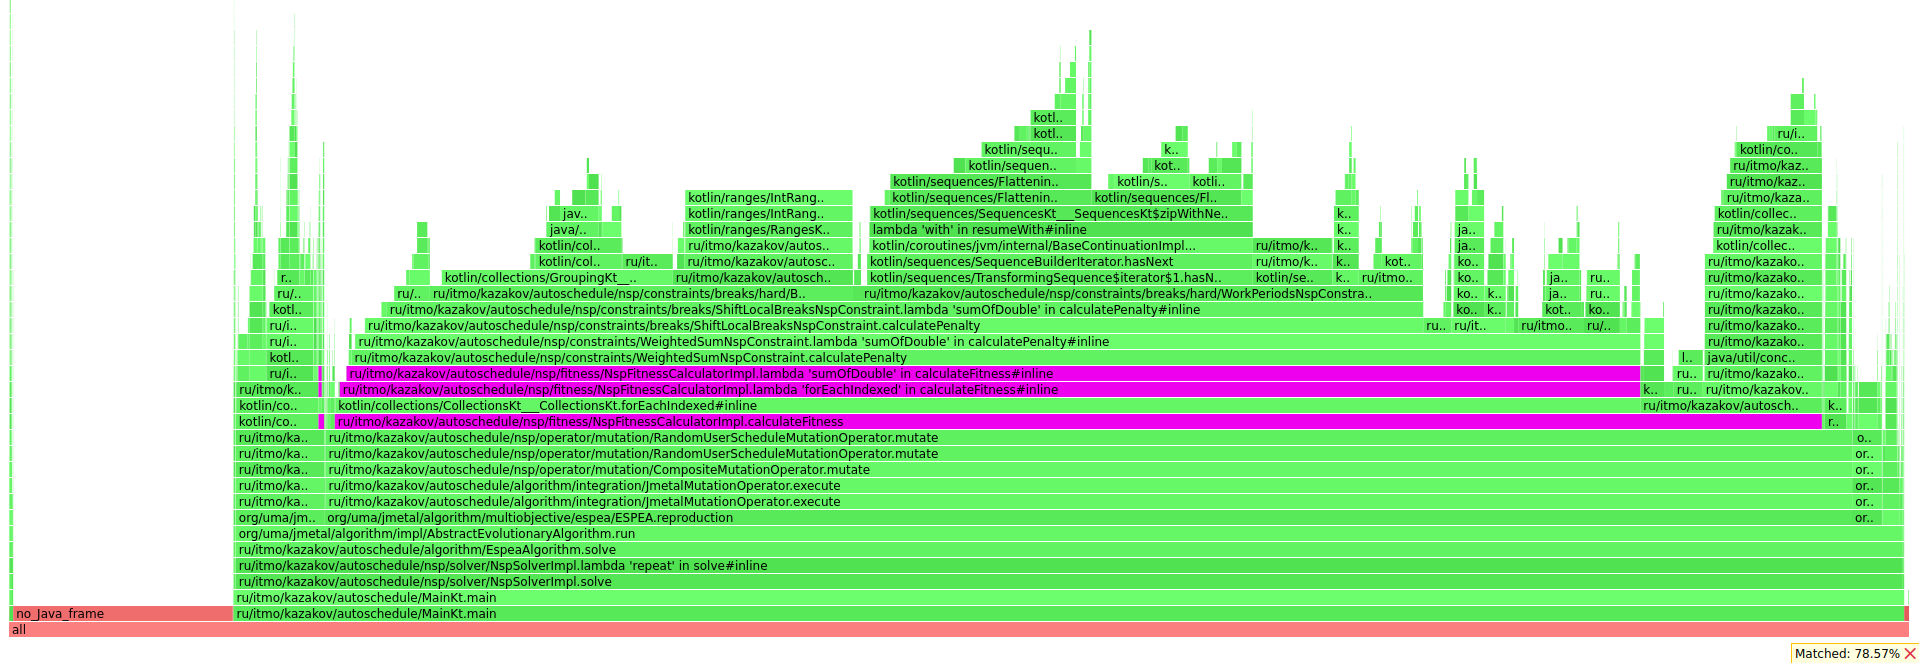
\includegraphics[width=1\columnwidth]{before_optimization_flame.png}
\end{figure}

На рисунке~\ref{fig2:flame_graph_before_optimization} представлен <<Граф пламени>> при запуске алгоритма на реальной команде техподдержки.
Фиолетовым цветом выделены вызовы, содержащие в себе подстроку <<calculateFitness>>~--- пересчет функции приспособленности.
Отсюда видно, что как раз его и надо оптимизировать.
Заметим, что пересчет штрафа~--- детерминированная функция.
Для одного и того же расписания оператора всегда будет один и тот же штраф.
Также заметим, что операторы мутации меняют расписания только одного оператора, поэтому переиспользование прошлых штрафов для пересчета новых может сильно ускорить исполнение.
Рассмотрим варианты переиспользования результатов прошлых подсчетов:

\begin{enumerate}
    \item сохранение результатов функции по каждым входным значениям с помощью шаблона проектирования <<декоратор>>;
    \item сохранение результатов функций в модели расписания путем добавления нового поля.
\end{enumerate}

Рассмотрим отличительные особенности первого подхода:

\begin{enumerate}
    \item необходимо следить за потреблением памяти~--- удалять устаревшие данные либо по истечению времени, либо по переполнению используемой структуры данных;
    \item простейшая реализация такого подхода использует ассоциативный массив в виде хеш-таблицы~--- для эффективного использования такого подхода нужно уметь быстро сравнивать расписания, а такая задача довольно нетривиальна;
    \item тем не менее, такой подход очень удобен~--- для реализации шаблона <<декоратор>> можно использовать аспектно-ориентированное программирование и помечать оптимизируемые функции аннотациями.
\end{enumerate}

Также рассмотрим отличительные особенности второго подхода:

\begin{enumerate}
    \item необходимо самостоятельно заполнять структуру данными, примененить аспектно-ориентированный подход значительно сложнее;
    \item в неизменяемой модели расписания появляется изменяемый ассоциативный массив~--- необходимо решать проблемы синхронизации потоков;
    \item для модели нужно инициализировать структуру для каждого нового объекта~--- если объекты ранее встречались, старую структуру сложно переиспользовать;
    \item тем не менее, нет необходимости следить за утечками памяти~--- при сборке мусора удалятся неиспользуемые объекты расписаний, а с ними удалятся и сохраненные данные.
\end{enumerate}

В конце концов, был выбран второй вариант, так как его использование влечет за собой менее ошибочный алгоритм.

Рассмотрим, как разработанный метод переиспользования вычислений можно применить к алгоритму планирования.
Оптимизировать будем пересчет штрафа, как уже было указано ранее.
Реализуем логику, которая будет вычислять разницу штрафа по каждому опрератору.
Тогда для неизменившихся расписаний можно брать штраф из построенной ранее структуры.
Для изменившихся смен будем использовать данные, посчитанные на прошлом шагу.
Для этого метод, пересчитывающий штраф, будет принимать список добавленных смен, удаленных смен, новое и старое расписания.
При использовании такого подхода, пересчет штрафа даже для большого расписания будет зависеть только от числа измененных смен.

Для штрафа за ограничения пересчет был оптимизирован тривиально: просто запустим подсчет штрафа по каждому оператору.
Несмотря на кажущуюся неоптимальность, такой подход позволяет пересчитывать штраф только для операторов, у которых изменилось расписание.
Дальнейшая оптимизация усложнит поддержку кода, поэтому не планируется ее проводить в ближайшее время.

Для пересчета штрафа покрытия прогноза на каждой итерации сохраняется покрытие прогноза по каждому шагу.
Тогда можно тривиально добавить и удалить смены к покрытию и посчитать индекс дисперсии.
Также можно оптимизировать подсчет самого индекса дисперсии, не используя те шаги, в которых число смен не изменилось.
Такой подход, как и в прошлый раз, не был использован ради упрощения кода.
<<Граф пламени>> после применения такой оптимизации представлен на рисунке~\ref{fig2:flame_graph_after_optimization}.
Как видно, процент времени, уходящий на пересчет функции приспособленности, уменьшился примерно в два раза.

\begin{figure}
\caption{<<Граф пламени>> алгоритма после оптимизации}\label{fig2:flame_graph_after_optimization}
\centering
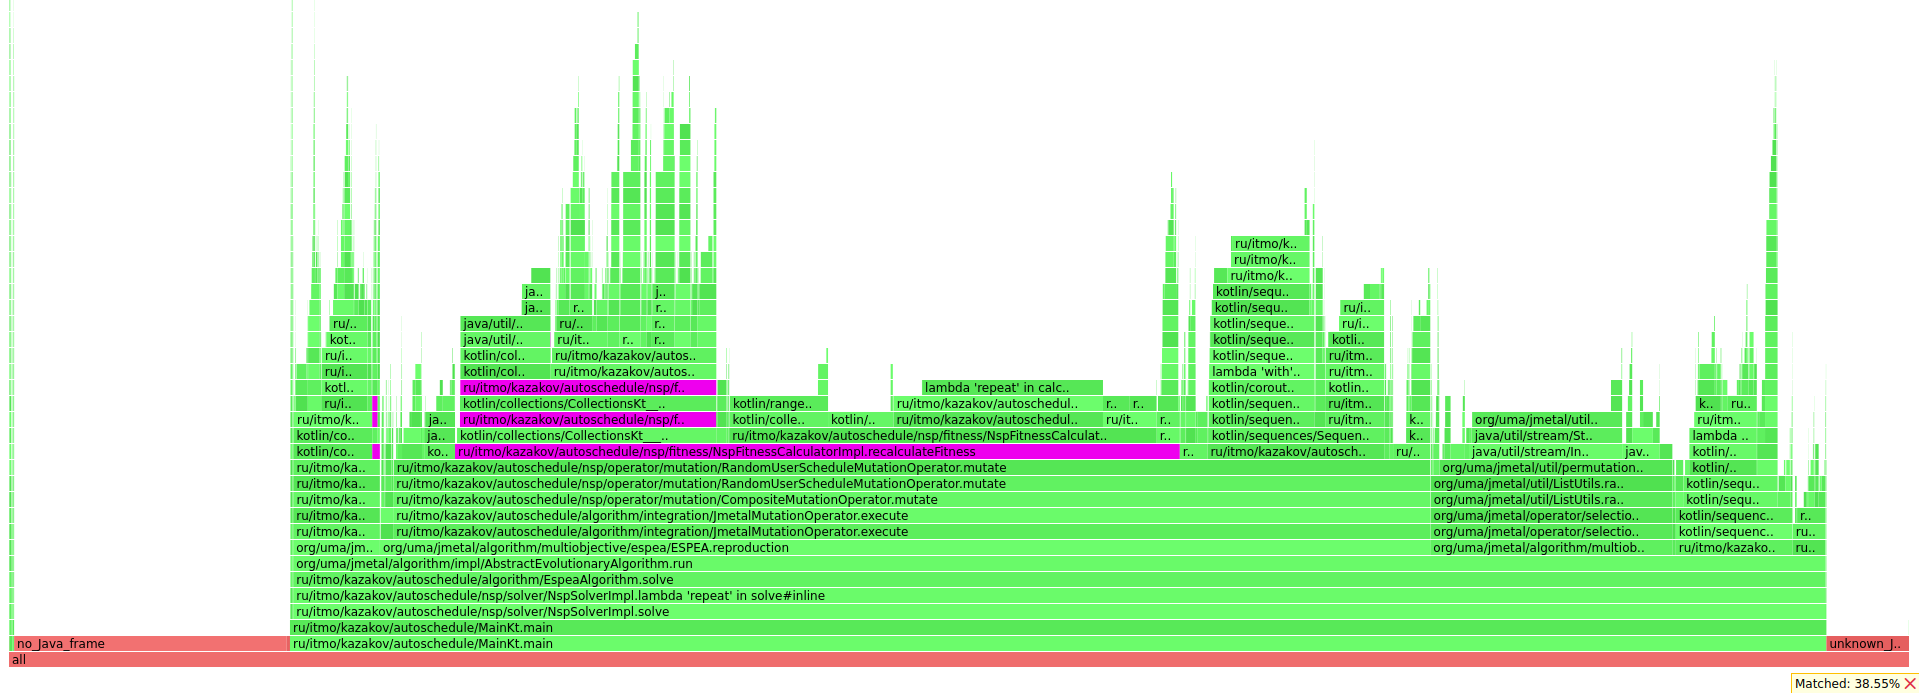
\includegraphics[width=1\columnwidth]{after_optimization_flame.png}
\end{figure}

\section{Сравнение алгоритмов планирования}

\subsection{Сравнение с решением задачи планирования дежурств медсестер}

Для начала сведем задачу к задаче квадратичного программирования.
Будем использовать способ аналогичный описанному в разделе~\ref{milp_and_miqp_subsection}.
Более подробно, опишем, как можно определить шаблоны смен в задаче планирования дежурств операторов служб поддержки.
В отличие от задачи планирования дежурств медсестер в шаблоны смен не заданы явно.
Тем не менее, их можно определить следующим образом: будем считать, что $t^i_{s, l, r}$~--- шаблон смены для $i$-го оператора длины $l$, который начинается с $s$-го допустимого начала смены оператора и имеет перерывы во время шагов из множества $r$.
Пример шаблонов смен показан на рисунке~\ref{fig2:support_shift_templates}.

\begin{figure}
\caption{Шаблоны смен в задаче планирования смен операторов}\label{fig2:support_shift_templates}
\centering
\includesvg[width=0.5\columnwidth]{svg/my_shift_templates}
\end{figure}

Обозначим смену, соответствующую шаблону смены $t^i_{s, l, r}$, как $s^i_{s, l, r}$, а множество смен в расписании как $S$.
Тогда можно задать двоичные переменные $a^i_{s, l, r}$, следующим образом:

\begin{equation} a^i_{s, l, r} = \begin{cases} 1,\, s^i_{s, l, r} \in S \\ 0,\, \text{иначе} \\ \end{cases}\,. \end{equation}

Далее, для каждого ограничения запишем неравенство для задачи квадратичного программирования:

\begin{enumerate}
    \item максимальная и минимальная длина смены: пусть $S^{b, 1}$~--- множество шаблонов смен с недопустимой длиной, тогда добавим ограничение

    \begin{equation} \forall i, s, l, r, t^i_{s, l, r} \in S^{b, 1} : a^i_{s, l, r} = 0; \label{nsp_reduction_filter_variables_1}\end{equation}

    \item дни начала всех смен одного оператора в его часовом поясе различны: пусть $D(s^i_{s, l, r})$~--- день начала смены $s^i_{s, l, r}$ в часовом поясе оператора $i$, а $S^{D, d, i} = \{ (s, l, r) \mid D(s^i_{s, l, r}) = d\}$, тогда добавим ограничение

    \begin{equation} \forall d, i : \sum\limits_{(s, l, r) \in S^{D, d, i}} a^i_{s, l, r} \le 1; \end{equation}

    \item каждая смена должна пересекаться с горизонтом планирования: пусть $S^{b, 2}$~--- множество шаблонов смен не пересекающихся с горизонтом планирования, тогда добавим ограничение

    \begin{equation} \forall i, s, l, r, t^i_{s, l, r} \in S^{b, 2} : a^i_{s, l, r} = 0; \label{nsp_reduction_filter_variables_2}\end{equation}

    \item суммарная длина всех смен должна быть равна норме: пусть $N_i$~--- норма оператора $i$, тогда добавим ограничение

    \begin{equation} \forall i : \sum\limits_{s, l, r} l a^i_{s, l, r} = N_i; \end{equation}

    \item смена оператора не должна пересекаться с отсутствием: пусть $S^{b, 3}$~--- множество шаблонов смен пересекающихся с отсутствиями, тогда добавим ограничение

    \begin{equation} \forall i, s, l, r, t^i_{s, l, r} \in S^{b, 3} : a^i_{s, l, r} = 0; \label{nsp_reduction_filter_variables_3}\end{equation}

    \item между сменами должен быть отдых (последовательные шаги, на которые оператор не назначен): пусть $R^{l, i}$~--- минимальная длина длина отдыха между сменами в шагах для оператора $i$, а также $R^{n, i}_{s, l, r} = \left\{ (s', l', r') \mid 0 \le s' - s < l + R^{l, i} \right\}$, тогда добавим ограничение

    \begin{equation} \forall i, s, l, r : \sum\limits_{(s', l', r') \in R^{n, i}_{s, l, r}} a^i_{s', l', r'} \le 1; \label{nsp_reduction_rest_constraint}\end{equation}

    \item смена оператора может начинаться только в заданные периоды начала смены: пусть $S^{b, 4}$~--- множество шаблонов смен, которые начинаются в недопустимые моменты, тогда добавим ограничение

    \begin{equation} \forall i, s, l, r, t^i_{s, l, r} \in S^{b, 4} : a^i_{s, l, r} = 0; \label{nsp_reduction_filter_variables_4}\end{equation}

    \item длины смен конкретного оператора не должны сильно различаться: пусть $N_i$ и $d_i$~--- норма оператора $i$ и число рабочих дней в планируемом периоде, тогда добавим ограничение

    \begin{equation} \forall i : \sum\limits_{s, l, r} a^i_{s, l, r} \left( l - \frac{N_i}{d_i} \right)^2 \rightarrow \min. \label{nsp_reduction_uniform_sizes}\end{equation}
\end{enumerate}

Заметим, что ограничения~\eqref{nsp_reduction_filter_variables_1},~\eqref{nsp_reduction_filter_variables_2},~\eqref{nsp_reduction_filter_variables_3} и~\eqref{nsp_reduction_filter_variables_4} могут быть применены на этапе построения сведения.
То есть алгоритм может использовать только те переменные $a^i_{s, l, r}$, для которых выполняются эти ограничения.
Аналогичным способом зададим ограничения на перерывы.
Если множество перерывов $r$ не удовлетворяет ограничениям, то не будем добавлять переменную $a^i_{s, l, r}$.

Также заметим, что ограничение~\eqref{nsp_reduction_uniform_sizes} нельзя тривиально добавить к ограничениям задачи линейного или квадратичного программирования.
В таком случае, ограничение~\eqref{nsp_reduction_uniform_sizes} необходимо добавить к оптимизируемой метрике.
В качестве оптимизируемой метрики возьмем дисперсию покрытия прогноза, к которой прибавим покрытие прогноза: пусть $p^i$~--- производительность оператора $i$, а $F_k$~--- прогноз для $k$-го шага, $D(X)$~--- несмещенная дисперсия списка $X$, тогда

\begin{equation} A_k = \sum\limits_{s \le k < s + l,\, k \notin r} p^i a^i_{s, l, r}; \; K_k = \frac{A_k}{F_k} \end{equation}

\begin{equation} P^f = D(K) + \sum\limits_{k} \frac{F_k - A_k}{F_k} \label{nsp_reduction_forecast_cover}\end{equation}

Так как $D(K)$ имеет в себе только квадратичные и линейные члены $A_k$, а $\sum\limits_{k} \frac{F_k - A_k}{F_k}$ содержит в себе только линейные члены $A_k$, то такая функция подходит для оптимизации целочисленным квадратичным программированием.
Сложив выражения~\eqref{nsp_reduction_forecast_cover} и~\eqref{nsp_reduction_uniform_sizes}, получим выражение, которое и будем оптимизировать целочисленным квадратичным программированием:

\begin{equation} F = P^f + \sum\limits_{i, s, l, r} a^i_{s, l, r} \left( l - \frac{N_i}{d_i} \right)^2 \end{equation}

К сожалению, такое сведение приводит к очень большому числу переменных $a^i_{s, l, r}$.
На практике число шаблонов смен достигает порядка 1~000~000.
Соответственно, матрица для такой задачи имеет размер порядка 1~000~000~x~1~000~000, что не вмещается в большинство современных устройств оперативной памяти.
Более того, из-за ограничения~\eqref{nsp_reduction_rest_constraint} число неравенств в сведении достигает таких же порядков, что и число переменных.

Таким образом, такое решение немасштабируемо и требует очень дорогих ресурсов для поддержки.
Поэтому такое решение не было выбрано в качестве основного.

\subsection{Применение других эволюционных алгоритмов}

Рассмотрим скорость сходимости разработанного алгоритма.
Сходимость зависит как от операторов мутации, так и от выбранного базового эволюционного алгоритма.
На рисунке~\ref{fig2:convergency_core_algorithms} представлено сравнение рассмотренных алгоритмов в данной работе.
По оси абсцисс указано время, за которое было получено решение с агрегированным штрафом, заданным по оси ординат.
Заметим, что указанное время не учитывает время генерации начальных решений.

\begin{figure}
\caption{Сходимость основных алгоритмов}\label{fig2:convergency_core_algorithms}
\centering
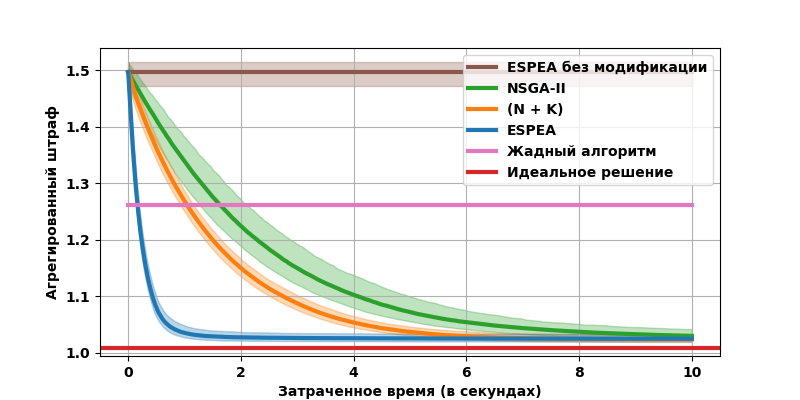
\includegraphics[width=1\columnwidth]{core_algorithms_convergency.png}
\end{figure}

Замеры проводились на компьютере с процессором Intel(R) Core(TM) i7-11850H @ 2.50ГГц и 32ГБ оперативной памяти.
Алгоритм запускался тысячу раз, принудительно останавливаясь через десять секунд после инициализации.
Предварительно алгоритм запускался один раз, чтобы виртуальная машина применила оптимизации времени исполнения к алгоритму.

Для замеров была выбрана типичная команда операторов службы поддержки из порядка тридцати операторов.
Расписание строилось на тридцать дней с шагом равным пятнадцати минутам.
В качестве прогноза было выбрано покрытие какого-то решения.
Более подробно, был взят прогноз из реальной службы поддержки и на нем было построено расписание с помощью алгоритма ESPEA.
Затем полученное расписание было взято как идеальное решение, которое идеально покрывает прогноз, то есть прогноз равен покрытию данного расписания.
Такой выбор прогноза позволяет оценить, насколько хорошо алгоритм приближает глобальный минимум.

Заметим, что выбранный алгоритм ESPEA показывает наилучшую сходимость среди всех рассмотренных алгоритмов.
Тем не менее, на графике видно, что алгоритм NSGA-II медленнее сходится к минимуму, чем алгоритм ($N + K$), хотя алгоритм NSGA-II также является многокритериальным.
При подробном исследовании этого вопроса было выяснено, что алгоритм ESPEA за тот же период успевает исполнить в $102.14 \pm 9.33$ раз больше итераций, чем NSGA-II.
Происходит это из-за того, что ESPEA основан на производительном быстром критерии выживания индивидуумов, чем NSGA-II.
Более того, ESPEA игнорирует такие решения, которые доминируются какими-то существующими, что позволяет быстро отбросить решения, движущиеся в неправильном направлении.

Также на графике видно, что алгоритм ($N + K$) сходится медленнее, чем ESPEA.
Это происходит из-за того, что алгоритм скаляризует функцию приспособленности, теряя информацию о каждой компоненте функции приспособленности.
Тем не менее данный алгоритм показывает неплохие результаты, имея сходимость лучше, чем у многих рассмотренных многокритериальных алгоритмов.
Такие результаты получились из-за того, что задача имеет довольно мало критериев.
Большинство ограничений выполняются для половины популяции, так как это гарантируется примененной модификацией.
Поэтому остаются только два содержательных критерия~--- критерий покрытия прогноза и критерий равномерности длин смен.
Второй критерий можно тривиально оптимизировать оператором мутации <<равномеризация смен>>, поэтому при достаточно большом числе итераций алгоритм превращается в однокритериальный.
Тем не менее, многокритериальный алгоритм позволяет развивать решение далее.
Например, скорее всего многокритериальный алгоритм будет иметь лучшую сходимость, чем у ($N + K$) при добавлении предпочтений операторов, как мягкое ограничение.

Также на графике представлено решение, основанное на алгоритме ESPEA и не использующее модификацию, описанную в разделе~\ref{section:used_evolutionary_algorithm_description}.
Заметим, что решения почти не улучшаются.
Такое поведение можно объяснить плохой выживаемостью хороших решений и малым разнообразием популяции.
Если наивно оценивать каждое решение, то окажется, что решения с небольшими нарушениями строгих ограничений довольно близки к решениям без таких нарушений.
Из-за этого алгоритмы, которые поддерживают равномерное распределение решений, не смогут поддерживать разнообразие среди допустимых решений.
Новые допустимые решения, скорее всего, будут удаляться, а старые будут неразнообразны.

Дополнительно, на графике представлено решение, полученное жадным алгоритмом.
Жадный алгоритм не улучшает решение постепенно, поэтому на графике он представлен горизонтальной прямой.
На рисунке~\ref{fig2:convergency_core_algorithms} видно, что эволюционные алгоритмы дают результаты лучше, чем жадный алгоритм.
На рисунке~\ref{fig2:forecast_cover_by_day} представлена метрика покрытия прогноза, замерявшаяся независимо для каждого дня в планируемом периоде.
Заметим, что эволюционный алгоритм статистически значимо лучше покрывает прогноз в каждый день.

\begin{figure}
\caption{Равномерность покрытия прогноза по каждому дню}\label{fig2:forecast_cover_by_day}
\centering
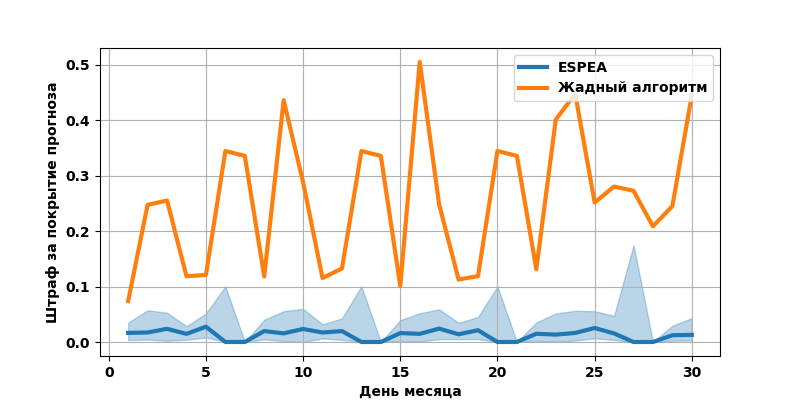
\includegraphics[width=1\columnwidth]{forecast_uniformity.png}
\end{figure}

Также заметим, что жадный алгоритм возвращает более оптимальное расписание, чем генераторы, используемые для эволюционных алгоритмов.
Тем не менее, жадный алгоритм генерирует решение $100.66 \pm 9.54$ секунд, а предложенный генератор создает расписание за $4.97 \pm 0.52$ миллисекунд.
Поэтому было принято решение взять быстрый генератор и исправить расписание эволюционным алгоритмом.

На рисунке~\ref{fig2:convergency_additional_algorithms} представлено сравнение дополнительно рассмотренных алгоритмов.
Для построения этого графика использовались аналогичные параметры, как и для построения графика на рисунке~\ref{fig2:convergency_core_algorithms}.
Также для сравнения на рисунок~\ref{fig2:convergency_additional_algorithms} был добавлен график сходимости алгоритма ESPEA.

\begin{figure}
\caption{Сходимость дополнительных алгоритмов}\label{fig2:convergency_additional_algorithms}
\centering
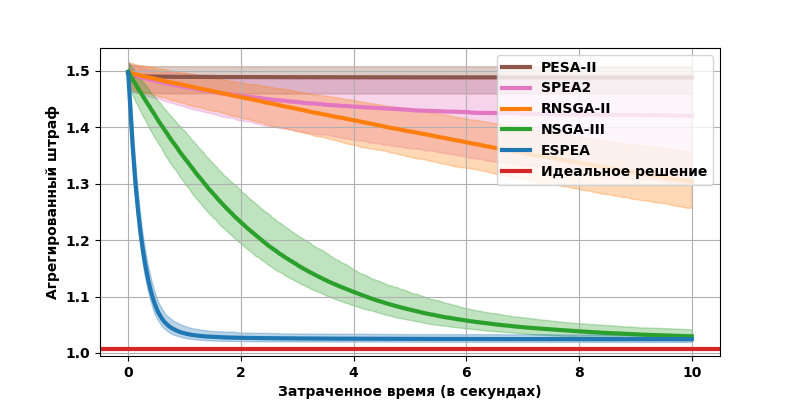
\includegraphics[width=1\columnwidth]{additional_algorithms_convergency.png}
\end{figure}

Заметим, что качество решения для алгоритмов PESA-II и SPEA2 довольно быстро выходит на плато, но полученное решение сильно хуже, чем решение алгоритмом ESPEA.
Более того, алгоритм PESA-II почти не улучшает решение~--- это связано с неудачным оператором выбора расписаний для мутации.
В этой выборке расписания очень часто повторяются, из-за чего не все решения доходят до этапа мутации.
Также на графике представлены алгоритмы RNSGA-II и NSGA-III.
Эти алгоритмы также не показали скорость сходимости, как у алгоритма ESPEA.
Как и в случае с NSGA-II, эти алгоритмы требуют много ресурсов процессора, из-за чего число итераций алгоритма ESPEA превосходит число итераций алгоритмов RNSGA-II и NSGA-III в несколько раз.

На рисунке~\ref{fig2:convergency_different_generators} представлена сходимость алгоритма ESPEA при выборе различных генераторов.

\begin{figure}
\caption{Сходимость алгоритма ESPEA при выборе различных генераторов}\label{fig2:convergency_different_generators}
\centering
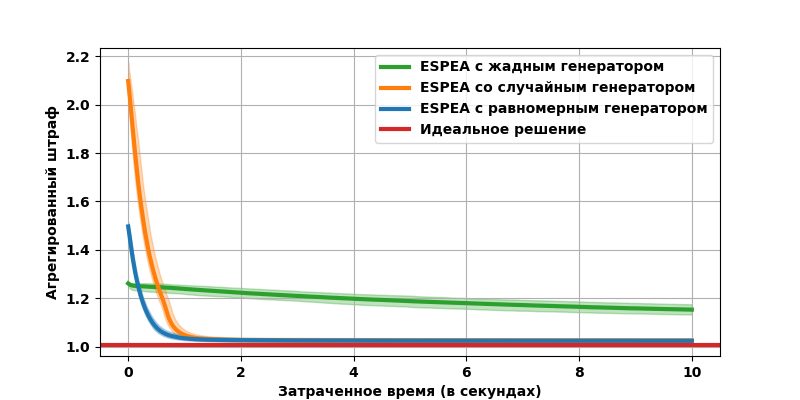
\includegraphics[width=1\columnwidth]{generators_algorithms_convergency.png}
\end{figure}

Заметим, что генератор, равномерно распределяющий смены по дням, лучше приблизил начальное решение к минимуму, чем случайный генератор.
Такое поведение наблюдается не только из-за того, что длины смен получаются равномерными, но и из-за того, что ресурс оператора более равномерно распределен по периоду планирования.
Тем не менее, оба генератора довольно быстро приводят алгоритм к сходимости, то есть имеет смысл использовать оба.

Жадный алгоритм хоть и предложил лучшее решение, эволюционный алгоритм ESPEA не смог его улучшить так, как смог улучшить решения остальных генераторов.
Такое поведение происходит из-за того, что жадный алгоритм генерирует расписания детерминированно, не используя генератор псевдослучайных чисел.
Из-за этого в начальной популяции есть только одно расписание, что подразумевает отсутствие разнообразия в ней.
А из-за отсутствия разнообразия алгоритм останавливается в одном локальном минимуме и не может найти альтернативные решения.

\chapterconclusion

Таким образом, был разработан программный код, который реализует описанный алгоритм.
Была описана архитектура приложения, а также рассмотрены возможные точки расширения.
Экспериментально было показано, что выбранный алгоритм решает задачу лучше остальных рассмотренных.
Было проведено сравнение с различными эволюционными алгоритмами, а также с жадным алгоритмом.
Также было описано сведение к задаче целочисленного квадратичиного программирования, которое на практике оказалось немасштабируемым.

В итоге, реализованный алгоритм был внедрен в компании Яндекс.

\startconclusionpage

В данной работе были рассмотрены ключевые особенности задачи планирования в службах поддержки.
Была найдена аналогичная сфера деятельности, имеющая схожие особенности~--- планирование дежурств медсестер.
Для задачи планирования в больницах были рассмотрены существующие решения, их преимущества и недостатки.
Были рассмотрены как алгоритмы, позволяющие разделить задачу планирования на две задачи, так и алгоритмы, полностью решающие данную задачу.

Также была подробно описана задача планирования смен операторов служб поддержки.
Были описаны все ограничения, поставленные в задаче, а также свойства, которые имеют операторы.
Далее были рассмотрены различия задачи планирования медсестер и операторов, описаны причины возникновения трудностей при использовании существующих решений.

Для решения задачи планирования операторов службы поддержки было предложено решение.
Была описана модификация классического эволюционного алгоритма, которая может улучшить сходимость алгоритма.
Для каждого описания была задана как оценка вектором чисел, так и численная оценка, которая позволяет сравнивать любые два решения.
Описаны генераторы начальных решений и операторы мутации, которые связали эволюционный алгоритм с решаемой задачей.
Предложенные компоненты были сравнены и был выбран теоретически лучший вариант.

В итоге, предложенный алгоритм был реализован, как библиотека программного обеспечения.
Была описана архитектура реализованной программы, рассмотрены точки развития.
Также были описаны возможности масштабирования алгоритма, которые позволяют планировать расписание в современных системах.

Реализованный алгоритм был сравнен с похожими решениями.
Было описано сведение к задаче квадратичного программирования, а также причины, почему оно немасштабируемо.
Для сравнений использовались как разные генераторы, так и разные эволюционные алгоритмы.
Также сравнение было проведено и с жадным алгоритмом.
Экспериментально было показано, почему разработанный алгоритм показывает лучшие результаты.

Разработанный алгоритм имеет огромный потенциал роста.
В проекте можно реализовать новые требования.
Например, можно планировать расписание для команд, в которых каждый оператор имеет множество навыков, а прогноз на каждый навык задан отдельно.
Также довольно просто можно добавить в алгоритм учет личных пожеланий операторов.

Таким образом, поставленная задача была решена.
Цель работы была достигнута, управление ресурсами служб поддержки было оптимизировано путем автоматизации планирования смен.
В итоге, данная работа была использована при внедрении в компании Яндекс.

\printmainbibliography


\end{document}



